\documentclass[12pt,onecolumn]{article}
\usepackage[utf8]{inputenc} % UTF8 input encoding
\usepackage[T2A]{fontenc}   % T2A font encoding for Cyrillic script
\usepackage[russian]{babel} % Russian language support
\usepackage{listings}
\usepackage{float}
\usepackage{mathtools}
\everymath{\displaystyle}
\usepackage{listings} 
\usepackage[usenames]{color}
\usepackage{geometry}
\usepackage{verbatim}
\usepackage{tabularray}
\usepackage{color}
\usepackage{longtable}
\usepackage{hyperref}
\newcommand{\nparagraph}[1]{\paragraph{#1}\mbox{}\\}
\geometry{
  a4paper,
  top=20mm, 
  right=25mm, 
  bottom=20mm, 
  left=20mm
}

\begin{document}
\setcounter{tocdepth}{4}
\begin{center}
    Федеральное государственное автономное образовательное учреждение высшего образования "Национальный Исследовательский Университет ИТМО"\\ 
    Мегафакультет Компьютерных Технологий и Управления\\
    Факультет Программной Инженерии и Компьютерной Техники \\
    
\includegraphics[scale=0.3]{image/itmo.jpg} % нужно закинуть картинку логтипа в папку с отчетом
\end{center}
\vspace{1cm}


\begin{center}
    \textbf{Лабораторная работа 3}\\
    \textit{"Локальные сети"}\\
    по дисциплине\\
    \textbf{Компьютерные сети}
\end{center}

\vspace{2cm}

\begin{flushright}
  Выполнил Студент  группы P33102\\
  \textbf{Лапин Алексей Александрович}\\
  Преподаватель: \\
  \textbf{Авксентьева Елена Юрьевна}\\
\end{flushright}

\vspace{6cm}
\begin{center}
    г. Санкт-Петербург\\
    2023г.
\end{center}

\newpage
\tableofcontents
\newpage

\section*{Цель работы}\addcontentsline{toc}{section}{Цель работы}
Изучение принципов конфигурирования и процессов функционирования компьютерных сетей, представляющих собой несколько подсетей, связанных с помощью маршрутизаторов, процессов автоматического распределения сетевых адресов, принципов статической маршрутизации и динамической маршрутизации, а также передачи данных на основе протоколов UDP и TCP.

В процессе выполнения лабораторной работы необходимо:

\begin{enumerate}
    \item построить модели компьютерных сетей, представляющих собой несколько подсетей, объединенных в одну автономную сеть, в соответствии с заданными вариантами топологий, представленными в Приложении (В1 -- В6);
    \item выполнить настройку сети при статической маршрутизации , заключающуюся в присвоении IP-адресов интерфейсам сети и ручном заполнении таблиц маршрутизации;
    \item промоделировать работу сети при использовании динамической маршрутизации на основе протокола RIP и при автоматическом распределении IP-адресов на основе протокола DHCP;
    \item выполнить тестирование построенных сетей путем проведения экспериментов по передаче данных на основе протоколов UDP и TCP;
    \item проанализировать результаты тестирования и сформулировать выводы об эффективности сетей с разными топологиями;
    \item сохранить разработанные модели локальных сетей для демонстрации процессов передачи данных при защите лабораторной работы.
\end{enumerate}
\section*{Вариант}
Вариант 4

P33102 Лапин Алексей Александрович

Ф = 5, И = 7, О = 13, Н = 2

Исходный адрес: $(7 + 2 + 128).(13+2).(5+2).(5+7) = 137.15.7.12 ... 137.15.7.21$
\section{ЗАДАНИЕ 1. Сеть с одним маршрутизатором (вариант В1)}
\subsection*{Построение и настройка сети с маршрутизатором.}
\begin{figure}[H]
    \centering
    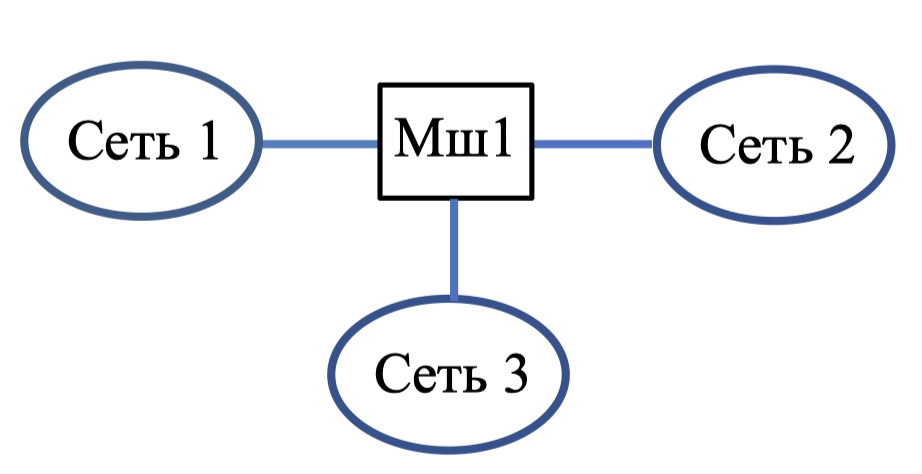
\includegraphics[width=0.5\textwidth]{image/part-1/task1.png}
    \caption{Вариант 1 построения КС}
\end{figure}
\begin{figure}[H]
    \centering
    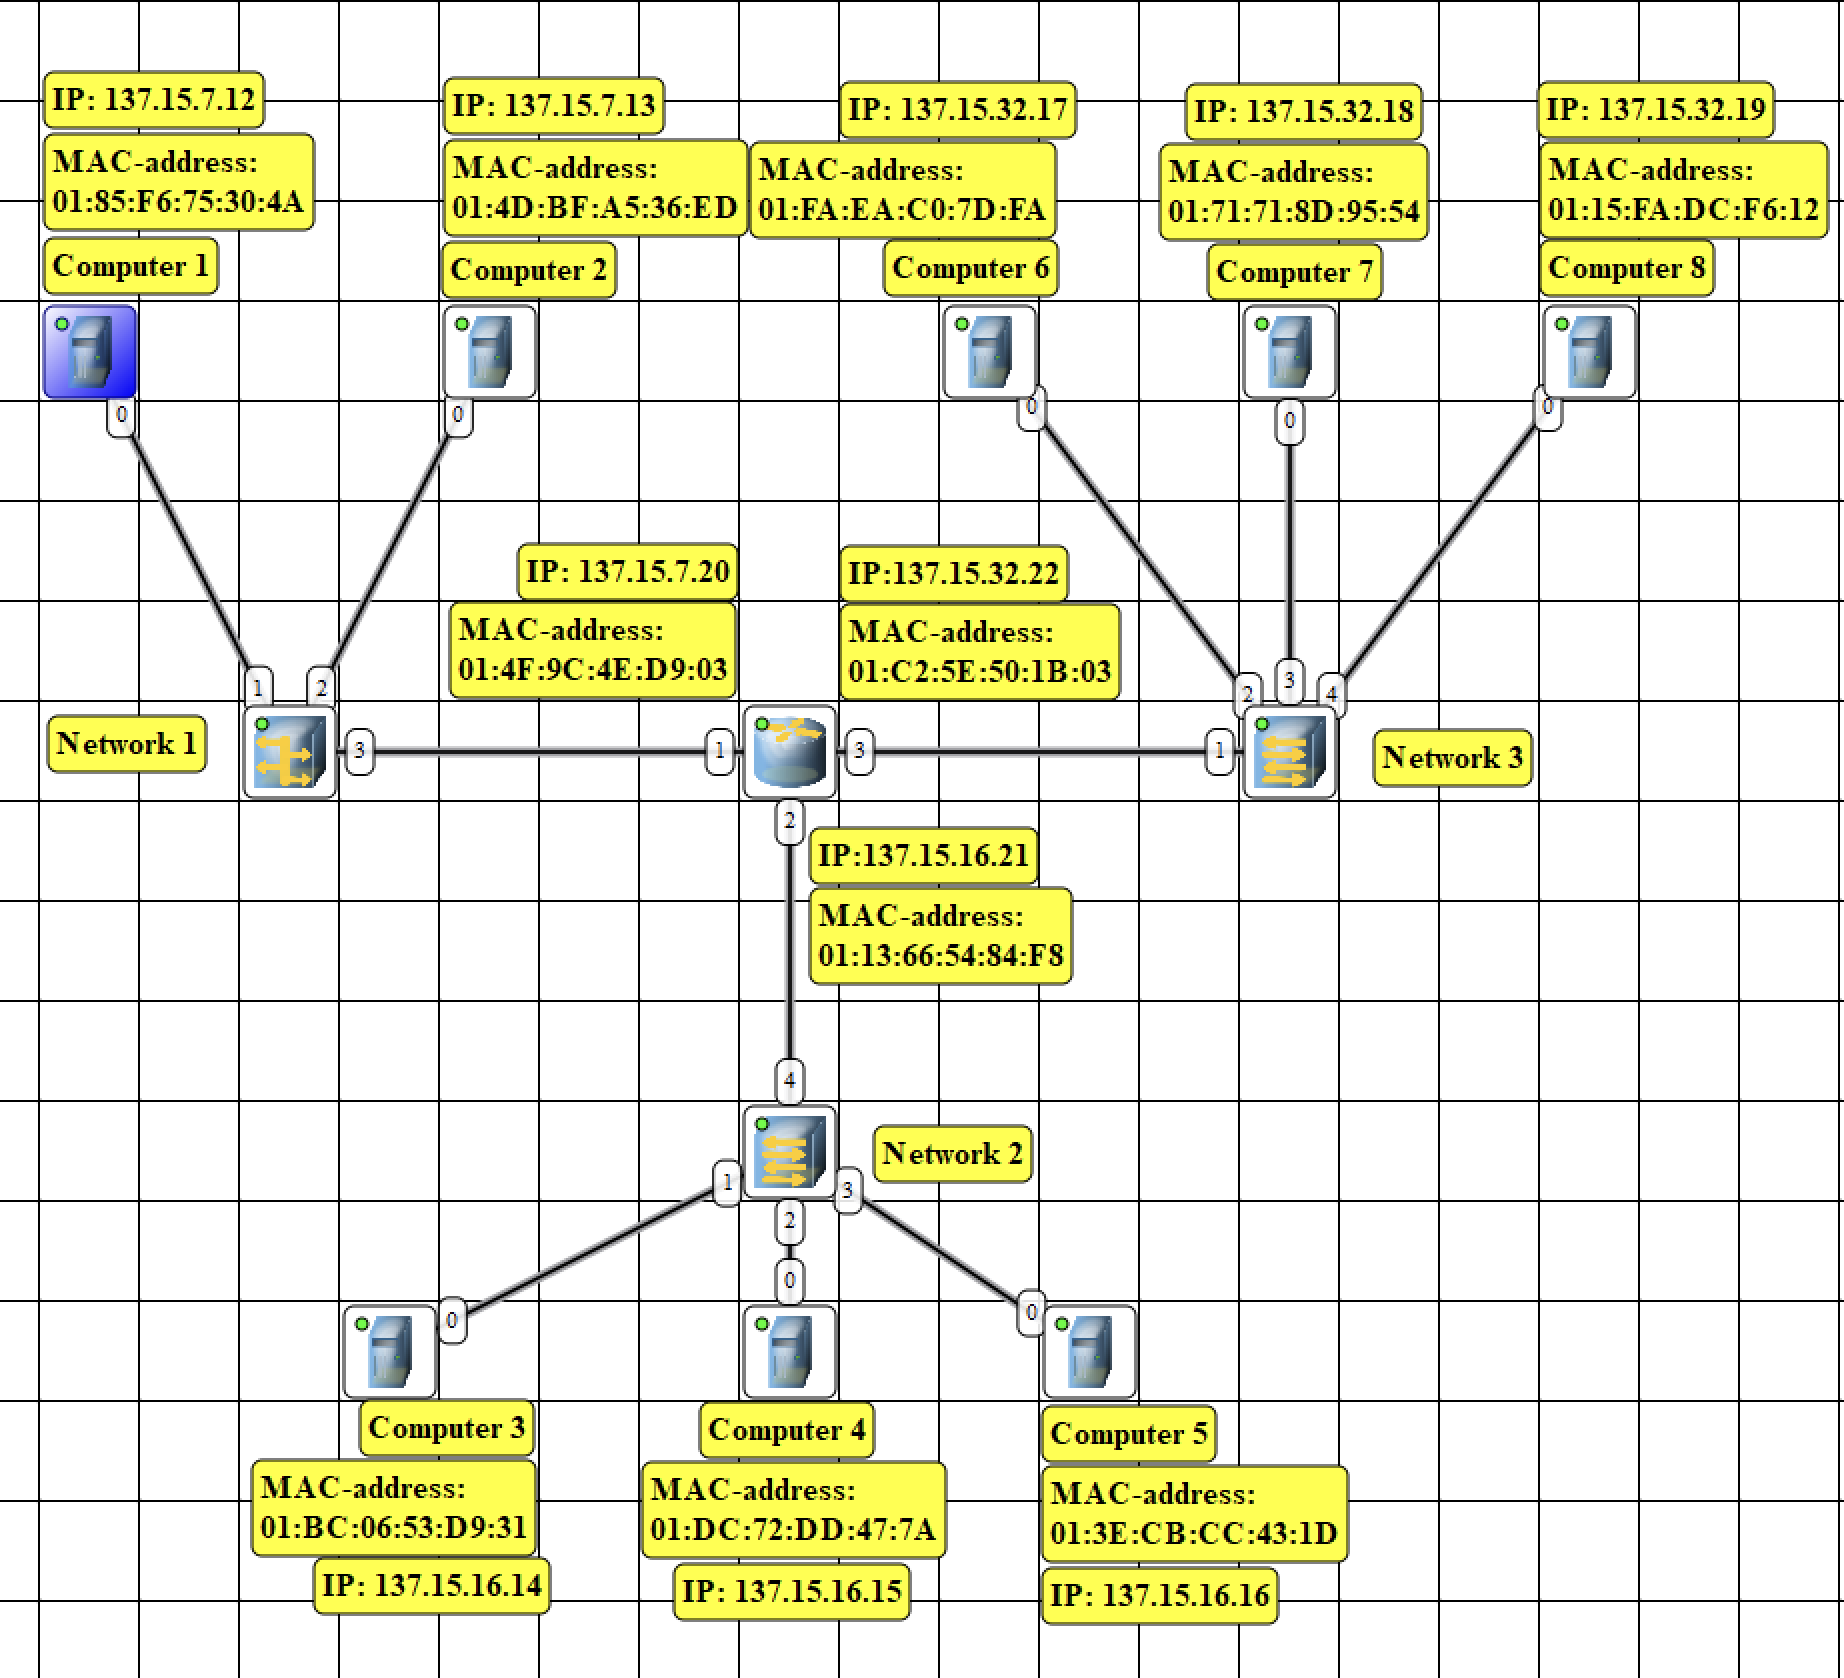
\includegraphics[width=\textwidth]{image/part-1/net1.png}
    \caption{Построенная сеть с одним маршрутизатором: В1}
\end{figure}
Для построения сети использовался пул адресов с 137.15.7.12
Адреса были выбраны таким образом, чтобы адрес сети класса B 
оставался таким же (маска 16 бит), а внутри неё выделялось некоторое количество подсетей.
Таким образом была выбрана маска 20 бит, которая дает возможность выделить 16 подсетей.
137.15.240.0 -- 137.15.250.0 для сети 137.15.0.0

Некоторые скриншоты, описывающие настройку сети:
\begin{figure}[H]
    \centering
    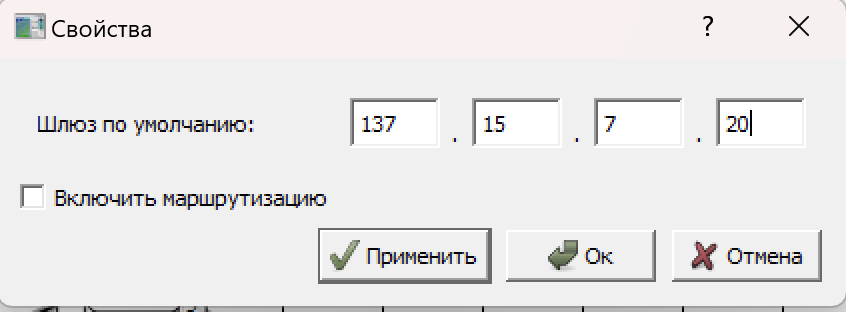
\includegraphics[width=0.3\textwidth]{image/part-1/default-gate.png}
    \caption{Шлюз по умолчанию для Компьютера 1}
\end{figure}
\begin{figure}[H]
    \centering
    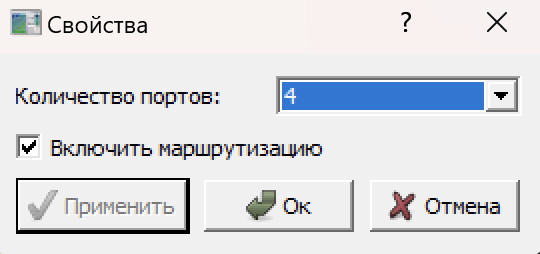
\includegraphics[width=0.3\textwidth]{image/part-1/router-settings.png}
    \caption{Настройки маршрутизатора}
\end{figure}
\begin{figure}[H]
    \centering
    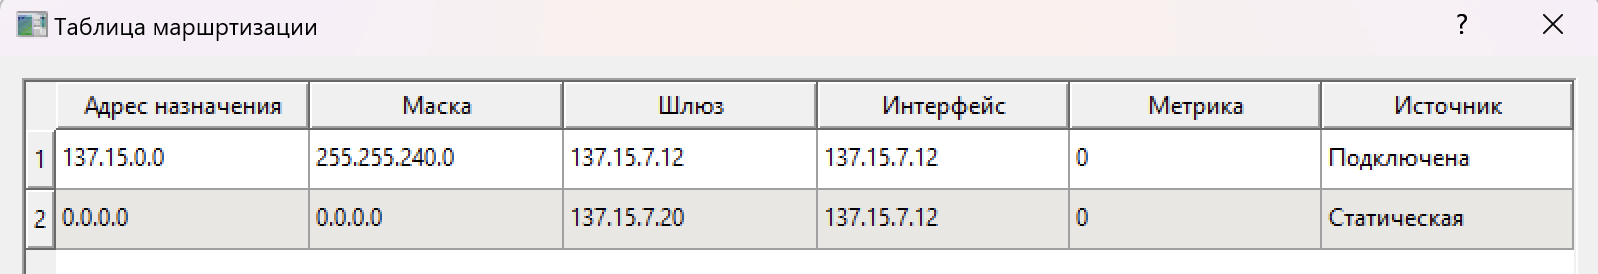
\includegraphics[width=\textwidth]{image/part-1/routung-table-1.png}
    \caption{Таблица маршрутизации Компьютера 1}
\end{figure}

В таблице маршрутизации компьютера находится 2 записи: первая запись -
запись для данной сети, предназначается для обмена пакетов в данной подсети,
вторая — шлюз по умолчанию, если адрес назначения из первой записи не
подходит, то есть адрес назначения не известен. Это потребуется, если
необходимо отправить данные на узел из другой подсети.

\begin{figure}[H]
    \centering
    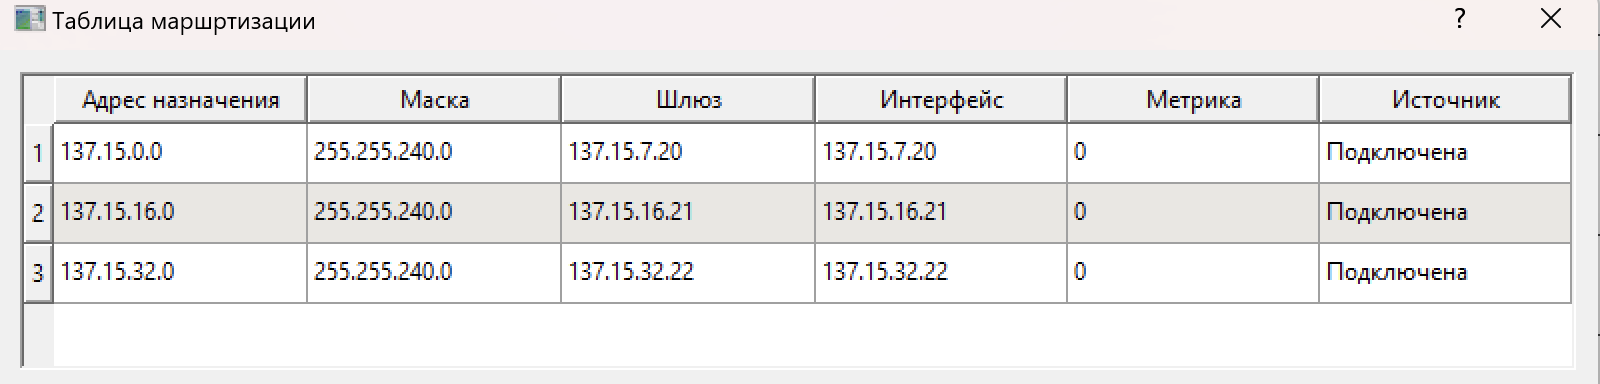
\includegraphics[width=\textwidth]{image/part-1/router-routing.png}
    \caption{Таблица маршрутизации маршрутизатора}  
\end{figure}


Здесь мы можем увидеть все три интерфейса для коммуникации с каждой из подсетей.

Таблица маршрутизации — это таблица данных, хранящаяся в маршрутизаторе, в которой перечислены маршруты к определенным сетевым пунктам назначения. Она содержит информацию о топологии сети непосредственно вокруг него.

В простейшем случае таблица состоит из адресов назначения, в соответствии которым ставится адрес следующего соседнего узла нашего маршрутизатора.

В нашем случае таблица маршрутизации состоит из следующих полей:
\begin{enumerate}
  \item Адрес назначения -- адрес подсети, к которой относится маршрут.
  \item Маска -- маска подсети для определения адресов узлов в данной сети.
  \item Адрес и маска подсети вместе задают адреса подсети.
  \item Интерфейс -- адаптор, на который нужно отправлять пакеты к указанной сети. (сетевые карты, обратная петля)
  \item Шлюз -- адрес маршрутизатора, через который нужно отправлять пакеты к указанной сети.
  \item Метрика --  определяет предпочтение для маршрута, когда есть варианты. Строчки с наименьшей метрикой предпочтительны при совпадении диапазонов.
  \item Источник -- источник появления записи в таблице маршрутизации.
\end{enumerate}

\subsection*{Тестирование сети (отправка пакетов).}
\subsubsection*{UDP}
\begin{figure}[H]
    \centering
    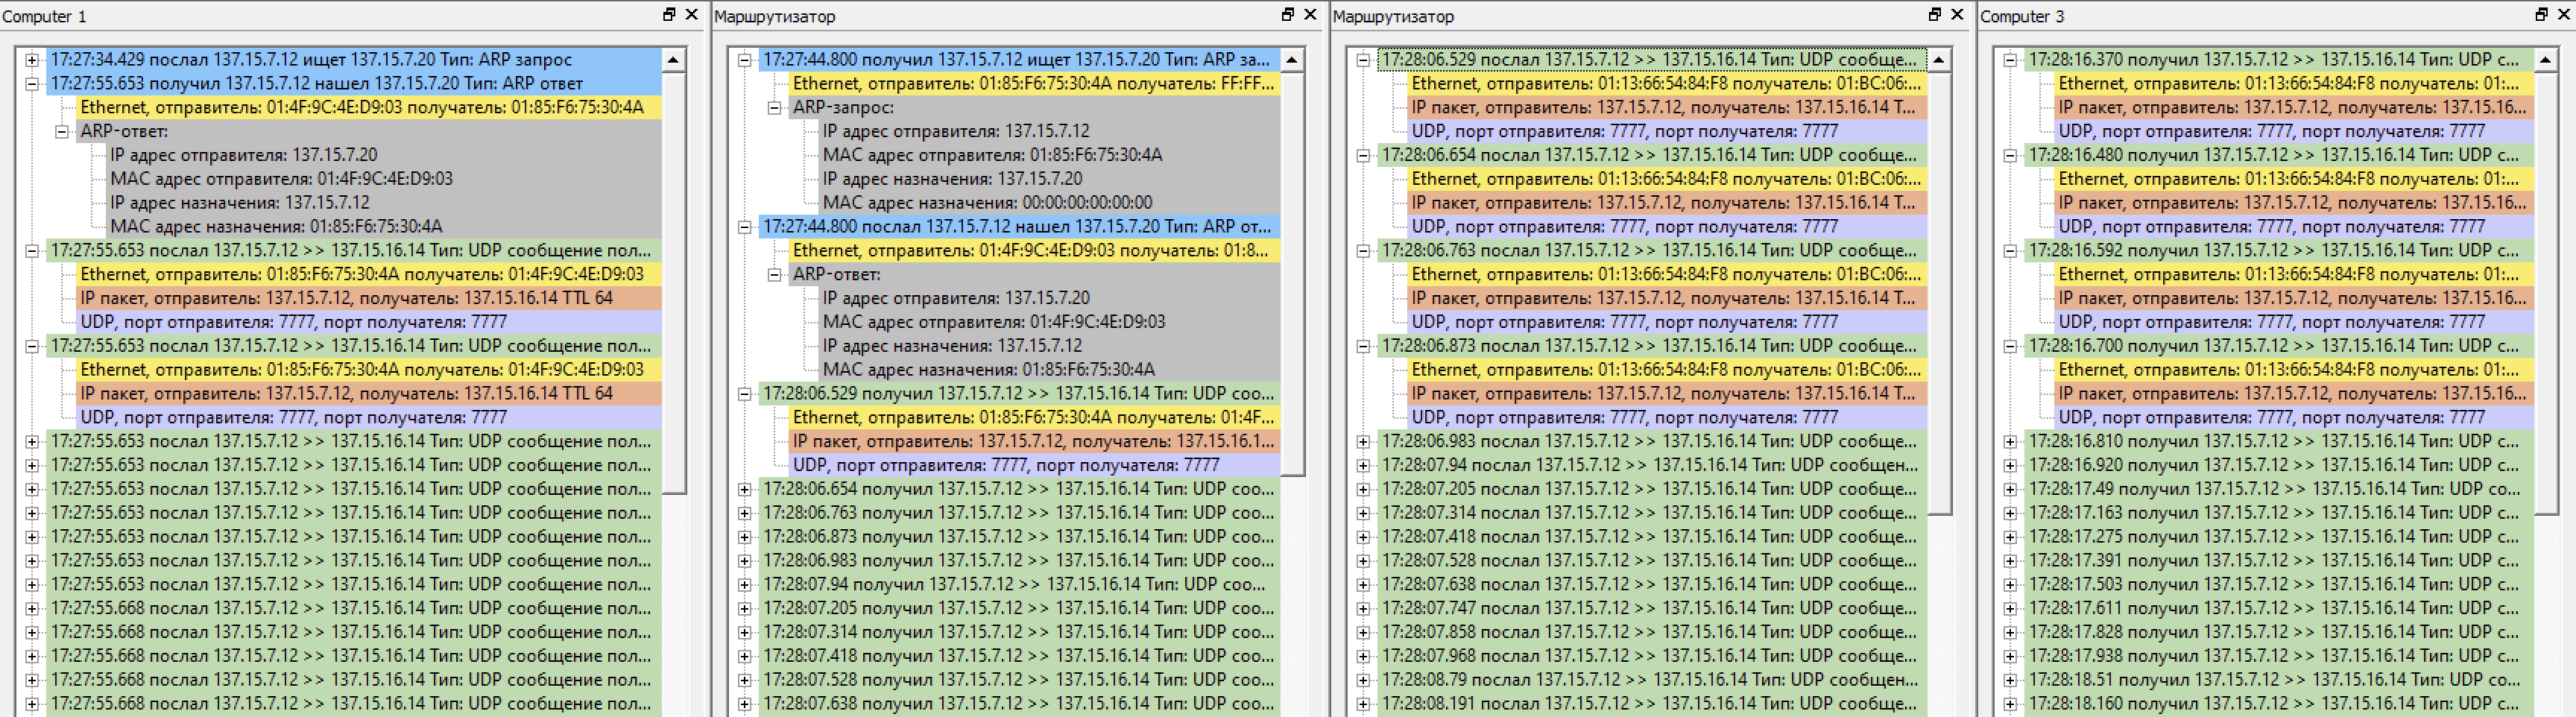
\includegraphics[width=\textwidth]{image/part-1/udp.png}
    \caption{Отправка UDP пакетов}
\end{figure}
Полный цикл отправки UDP-запроса:
\begin{enumerate}
    \item Компьютер определяет МАС-адреса маршрутизатора, отправляя ARP-запрос и получая ответ.
    \item Компьютер отправляет пакет, в котором в кадре Ethernet в качестве получателя указан не МАС-адрес компьютера-получателя, а маршрутизатора, LAN-1.
    \item Маршрутизатор отправляет ответ на компьютер-получатель (предварительно узнав его МАС-адрес), при этом в качестве МАС-адреса отправителя указывает адрес сетевой карты маршрутизатора, а получателя – МАС-адрес компьютера (его сетевой карты).
\end{enumerate}
\subsubsection*{TCP}
\begin{figure}[H]
    \centering
    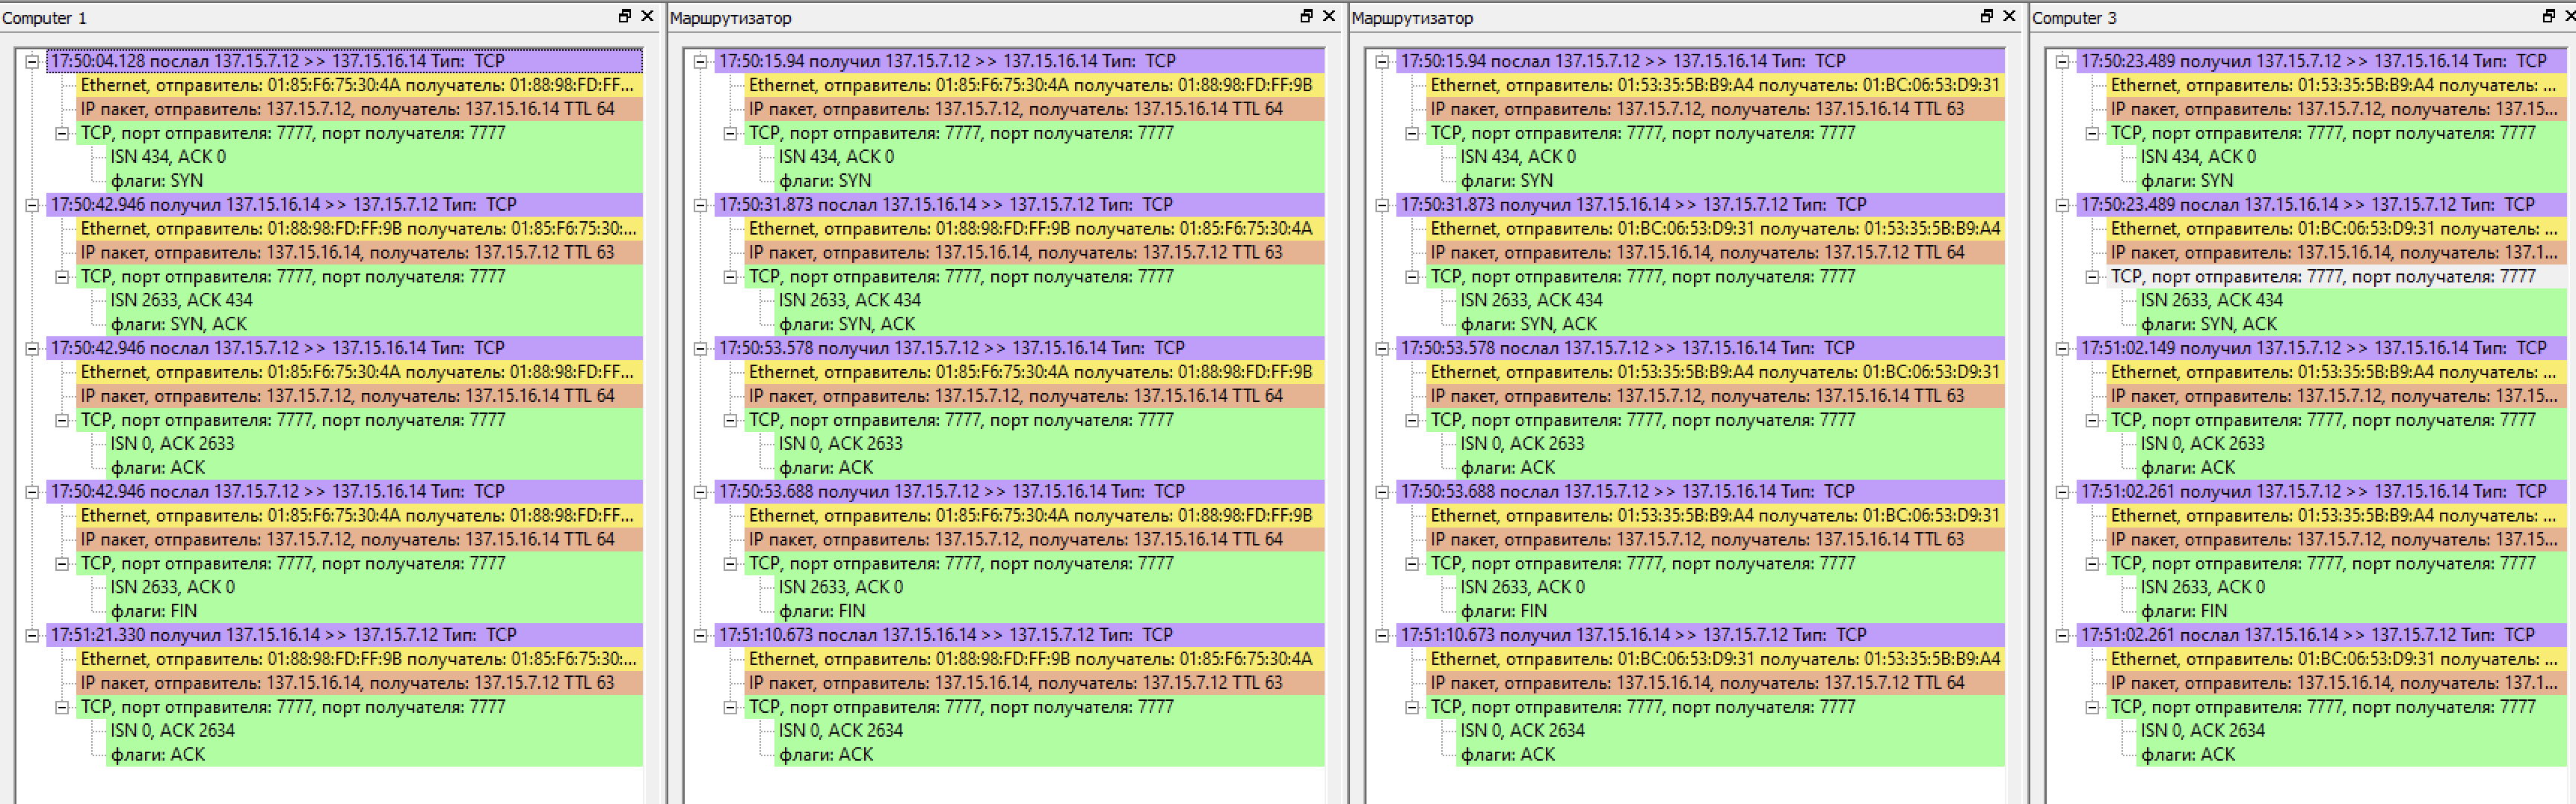
\includegraphics[width=\textwidth]{image/part-1/tcp.png}
    \caption{Отправка TCP пакетов}
\end{figure}
Для протокола ТСР, принцип установки адресов МАС аналогичен, а процесс тройного рукопожатия и подтверждения были детально описаны в предыдущей лабораторной работе.
\section{ЗАДАНИЕ 2. Сеть двумя маршрутизаторами (вариант В2)}
\subsection{Построение и настройка сети с двумя маршрутизаторами.}
\begin{figure}[H]
    \centering
    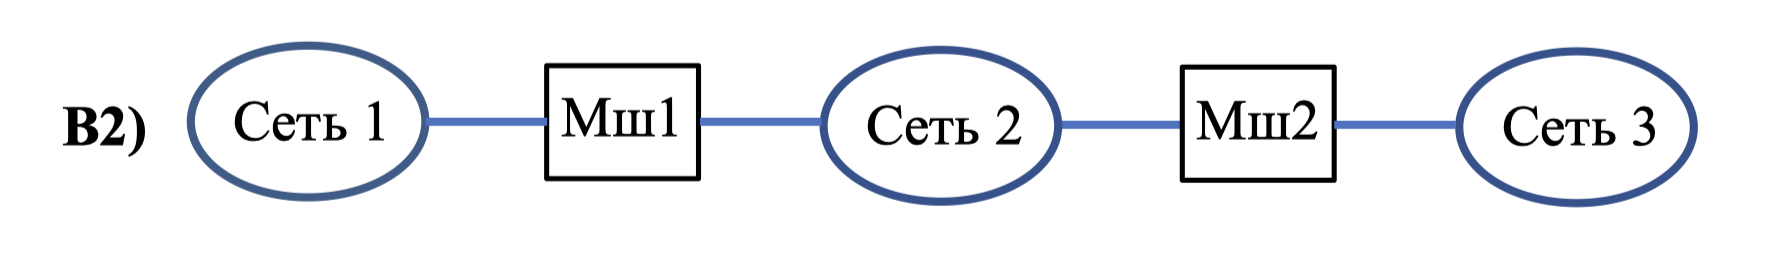
\includegraphics[width=0.5\textwidth]{image/part-2/task2.png}
    \caption{Вариант 2 построения КС}
\end{figure}
\begin{figure}[H]
    \centering
    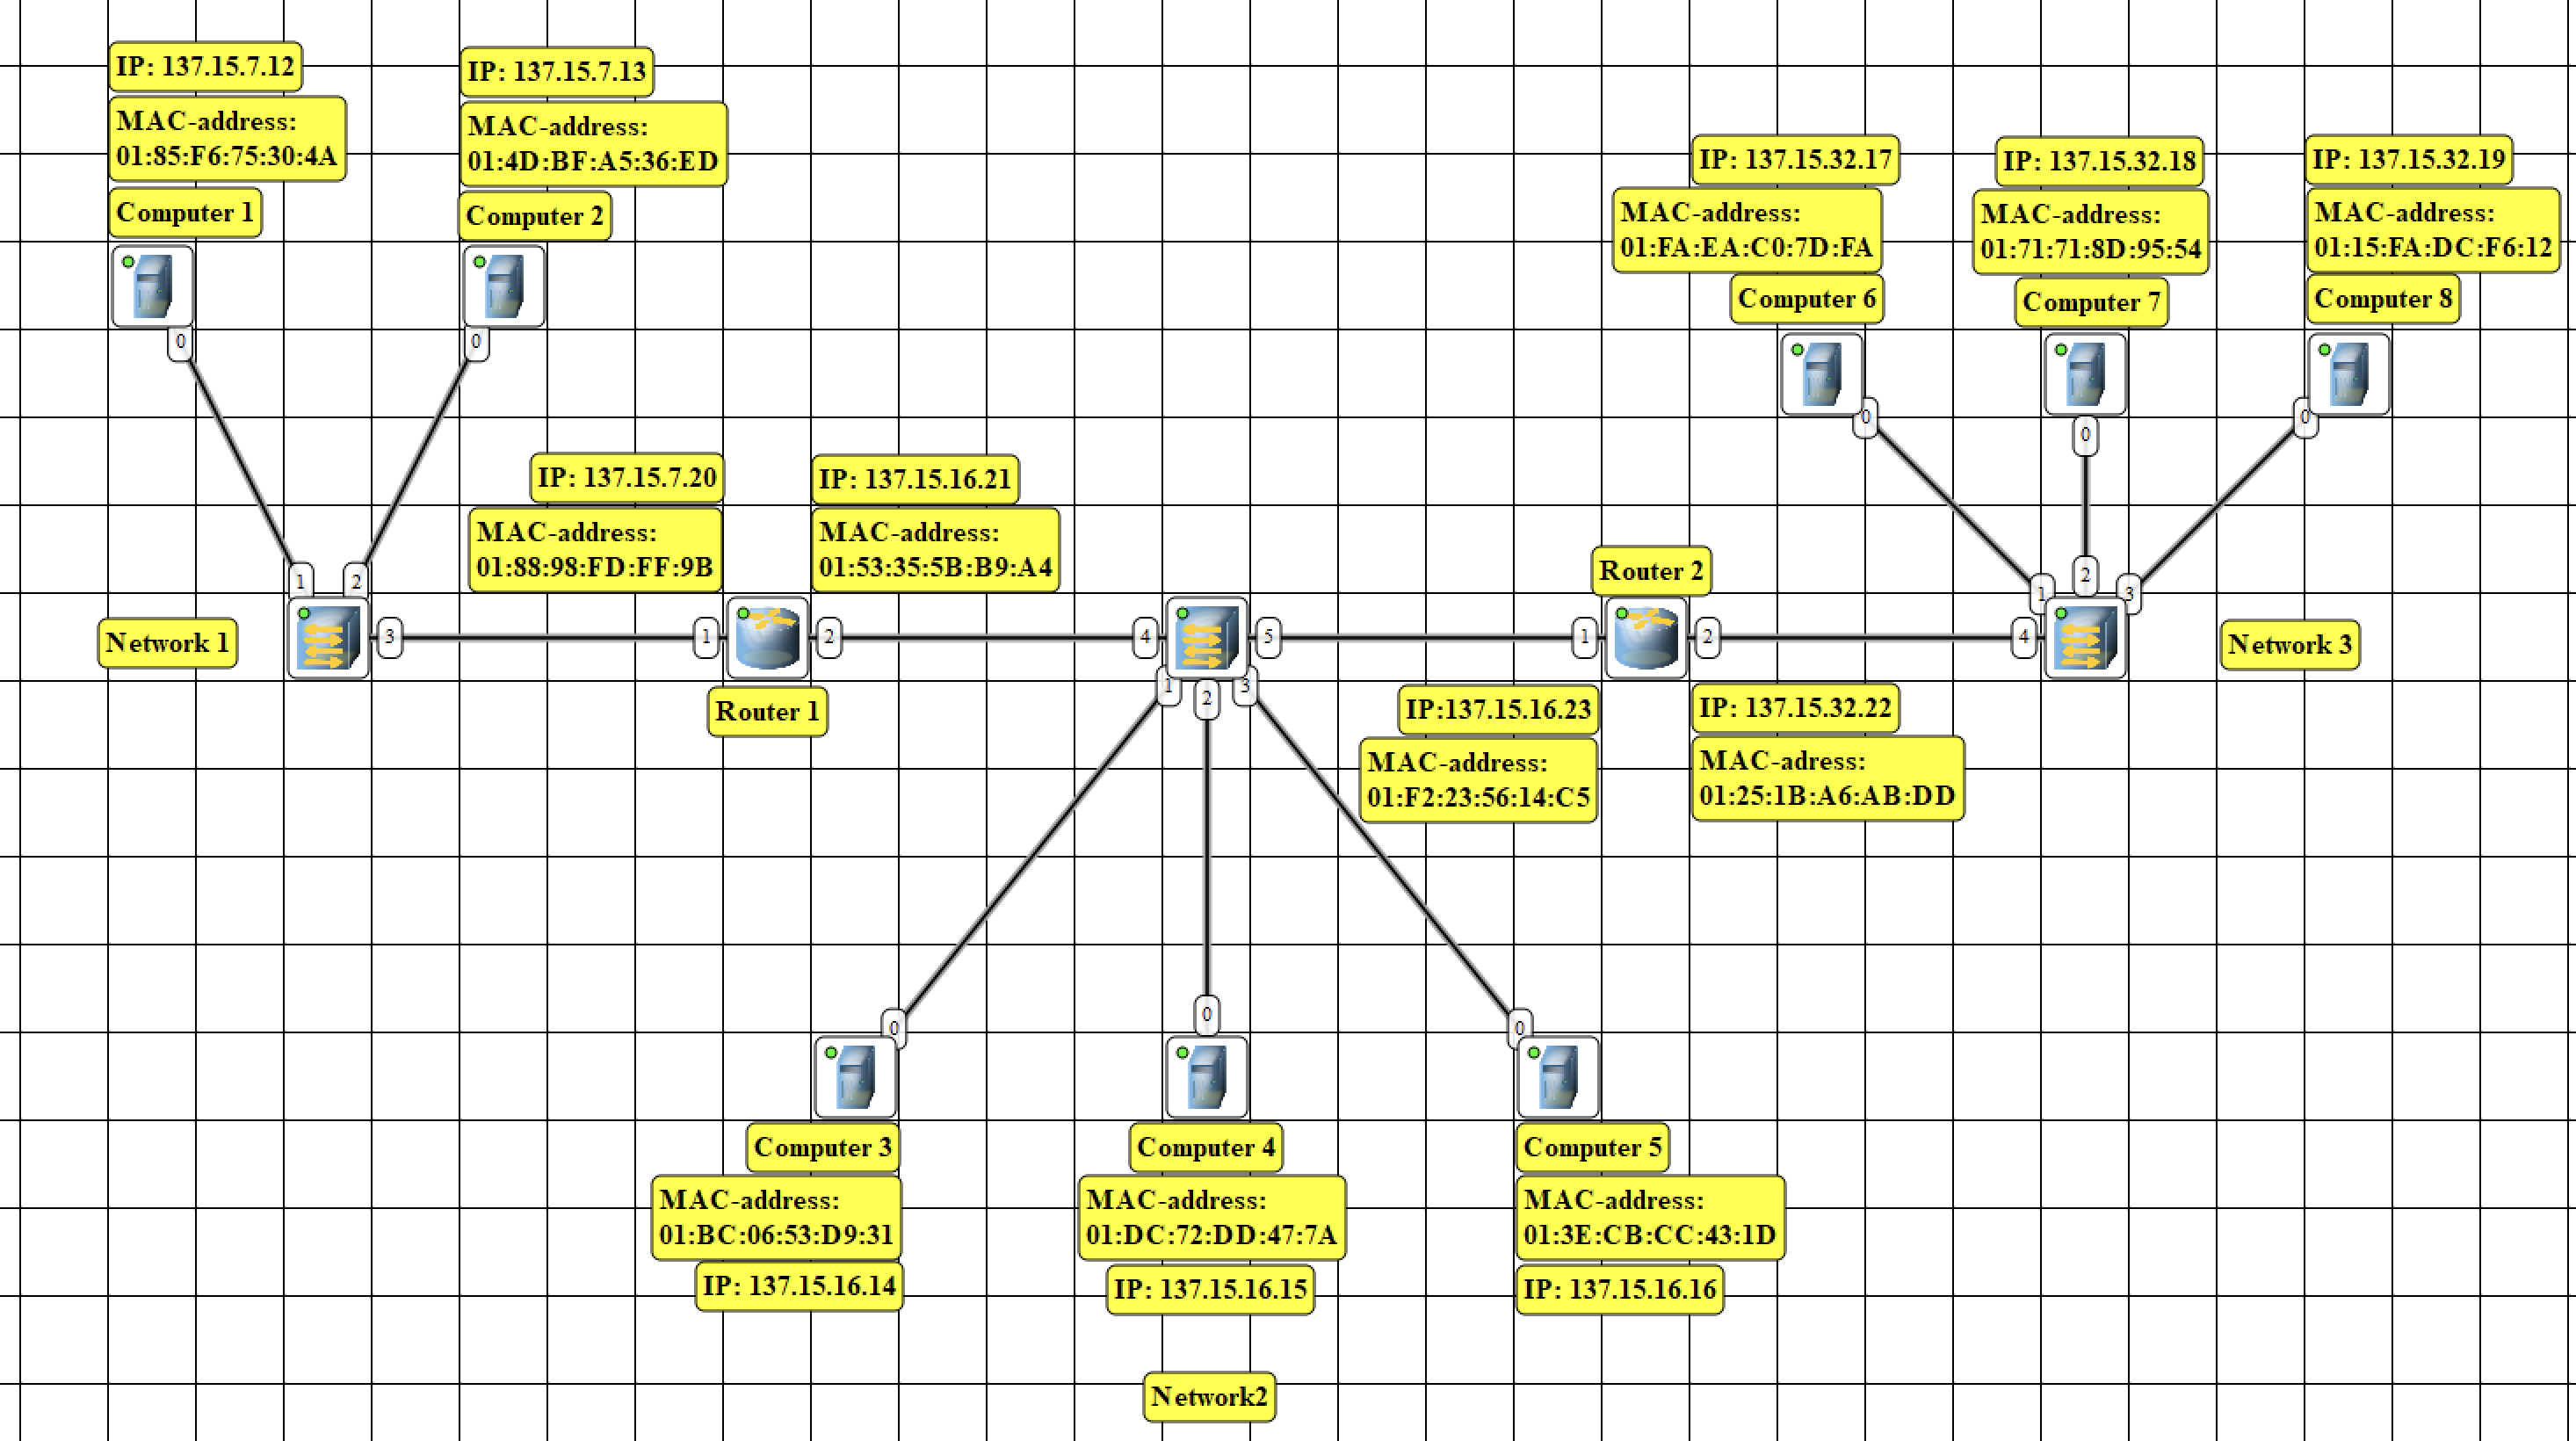
\includegraphics[width=\textwidth]{image/part-2/net2.png}
    \caption{Построенная сеть с двумя маршрутизаторами: В2}
\end{figure}
Состояние таблиц маршрутизации аналогично предыдущему случаю. 
Но надо подумать какими путями пойдут пакеты из сети 2.

Выставим шлюз по умолчанию на Router 1, потому что с ним связана подсеть с
меньшим кол-вом узлов, а значит он будет менее загружен.

\begin{figure}[H]
    \centering
    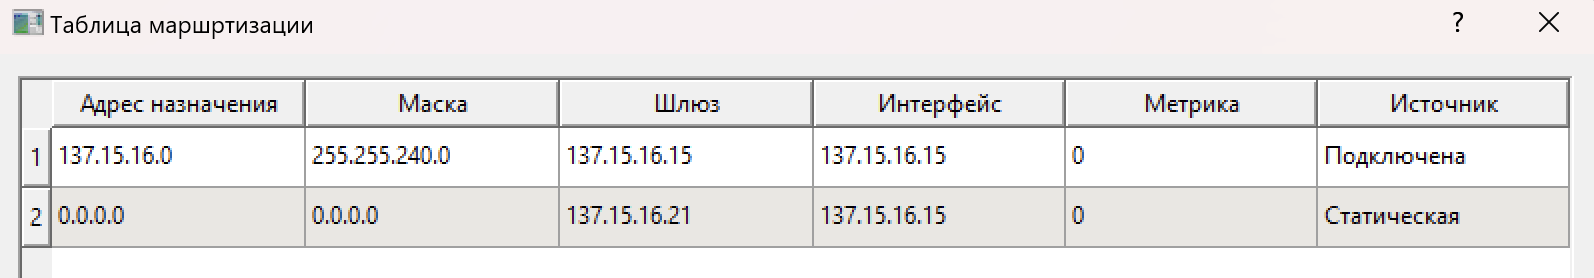
\includegraphics[width=\textwidth]{image/part-2/routing-computer4.png}
    \caption{Таблица маршрутизации Компьютера 4}
\end{figure}

В Router 2 сделаем запись (статическую), что пакеты должны пересылаться в подсеть 1, если их получатель находится там.
\begin{figure}[H]
    \centering
    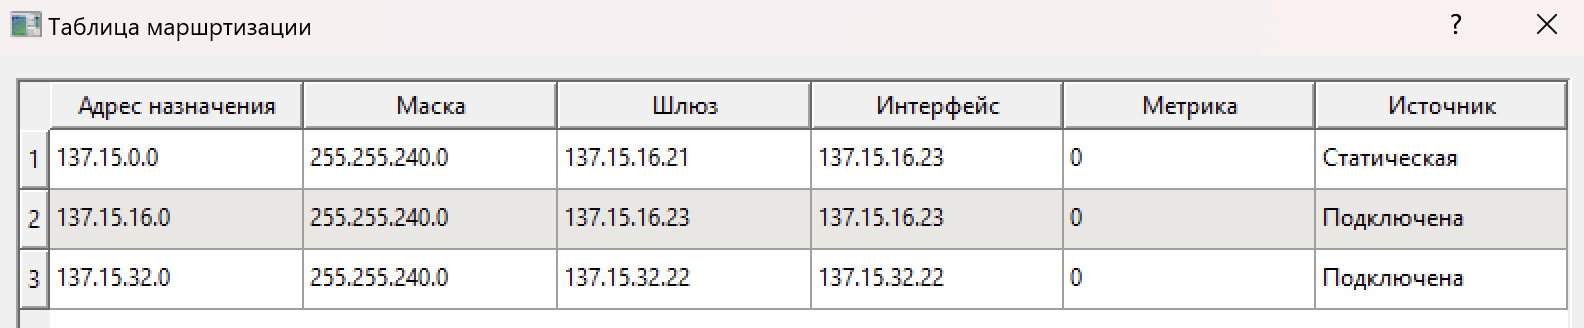
\includegraphics[width=\textwidth]{image/part-2/router2-routing.png}
    \caption{Таблица маршрутизации Router 2}
\end{figure}

В Router 1 занесем запись о получателя из подсети 3.
\begin{figure}[H]
    \centering
    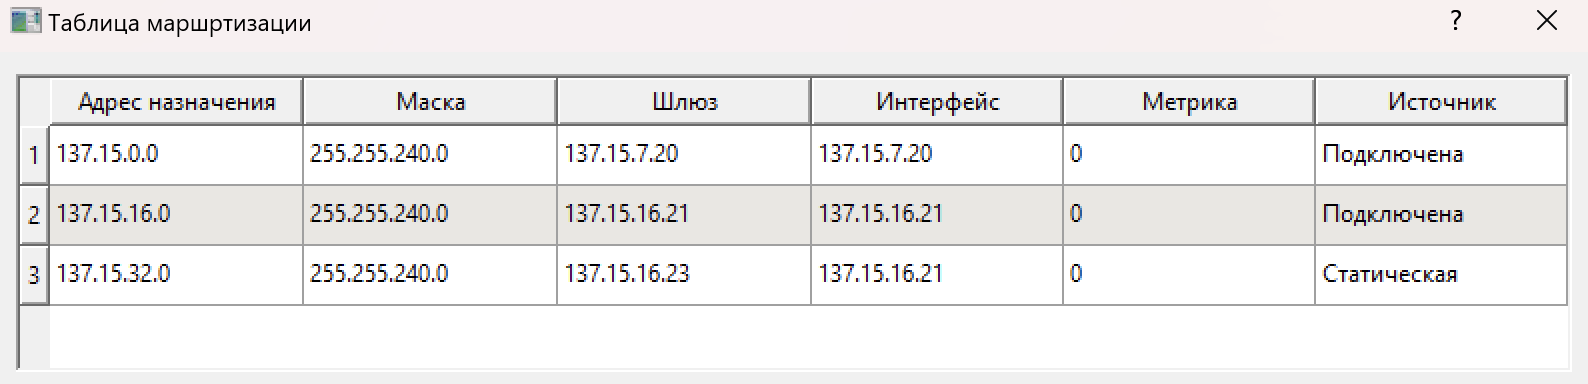
\includegraphics[width=\textwidth]{image/part-2/router1-routing.png}
    \caption{Таблица маршрутизации Router 1}
\end{figure}
\subsection{Тестирование сети (отправка пакетов).}
\subsubsection{UDP}
\begin{figure}[H]
    \centering
    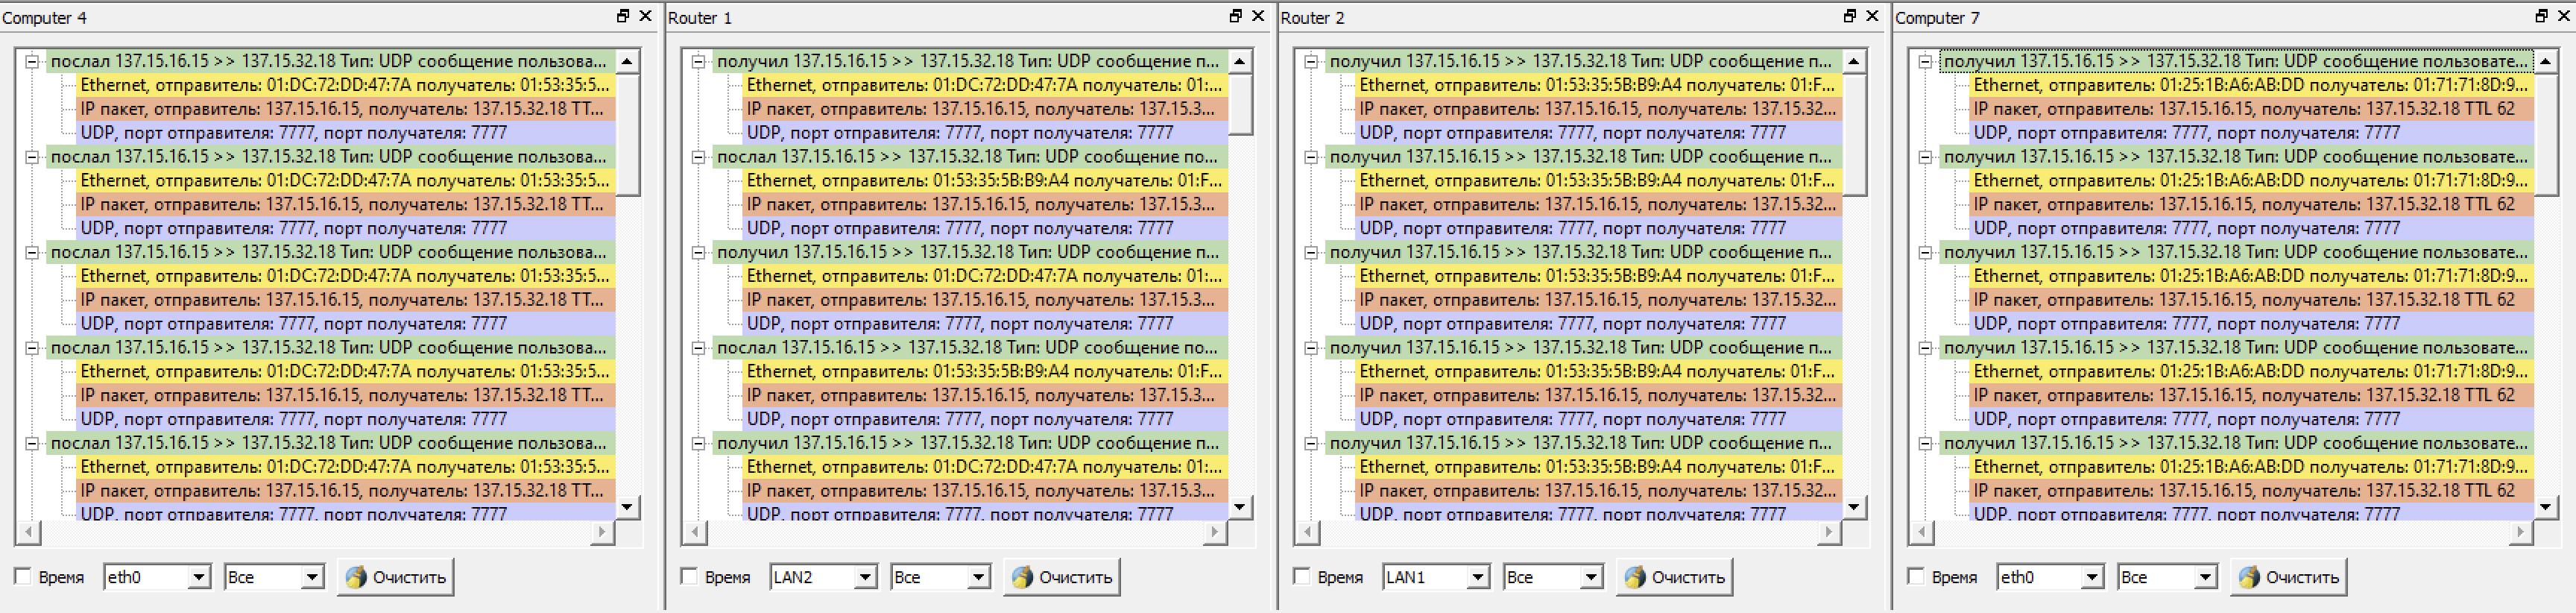
\includegraphics[width=\textwidth]{image/part-2/udp.png}
    \caption{Отправка UDP пакетов}
\end{figure}
Здесь продемонстрирована отправка пакетов из сети 2 в сеть 3.
Сначала пакеты будут отправлены на Router 1, а затем на Router 2, и только потом конечному получателю.

Подмена MAC-адреса отправителя в каждом маршрутезаторе на MAC-адрес сетевой карты маршрутизатора, была рассотрена в предыдущем пункте.

\subsubsection{TCP}
\begin{figure}[H]
    \centering
    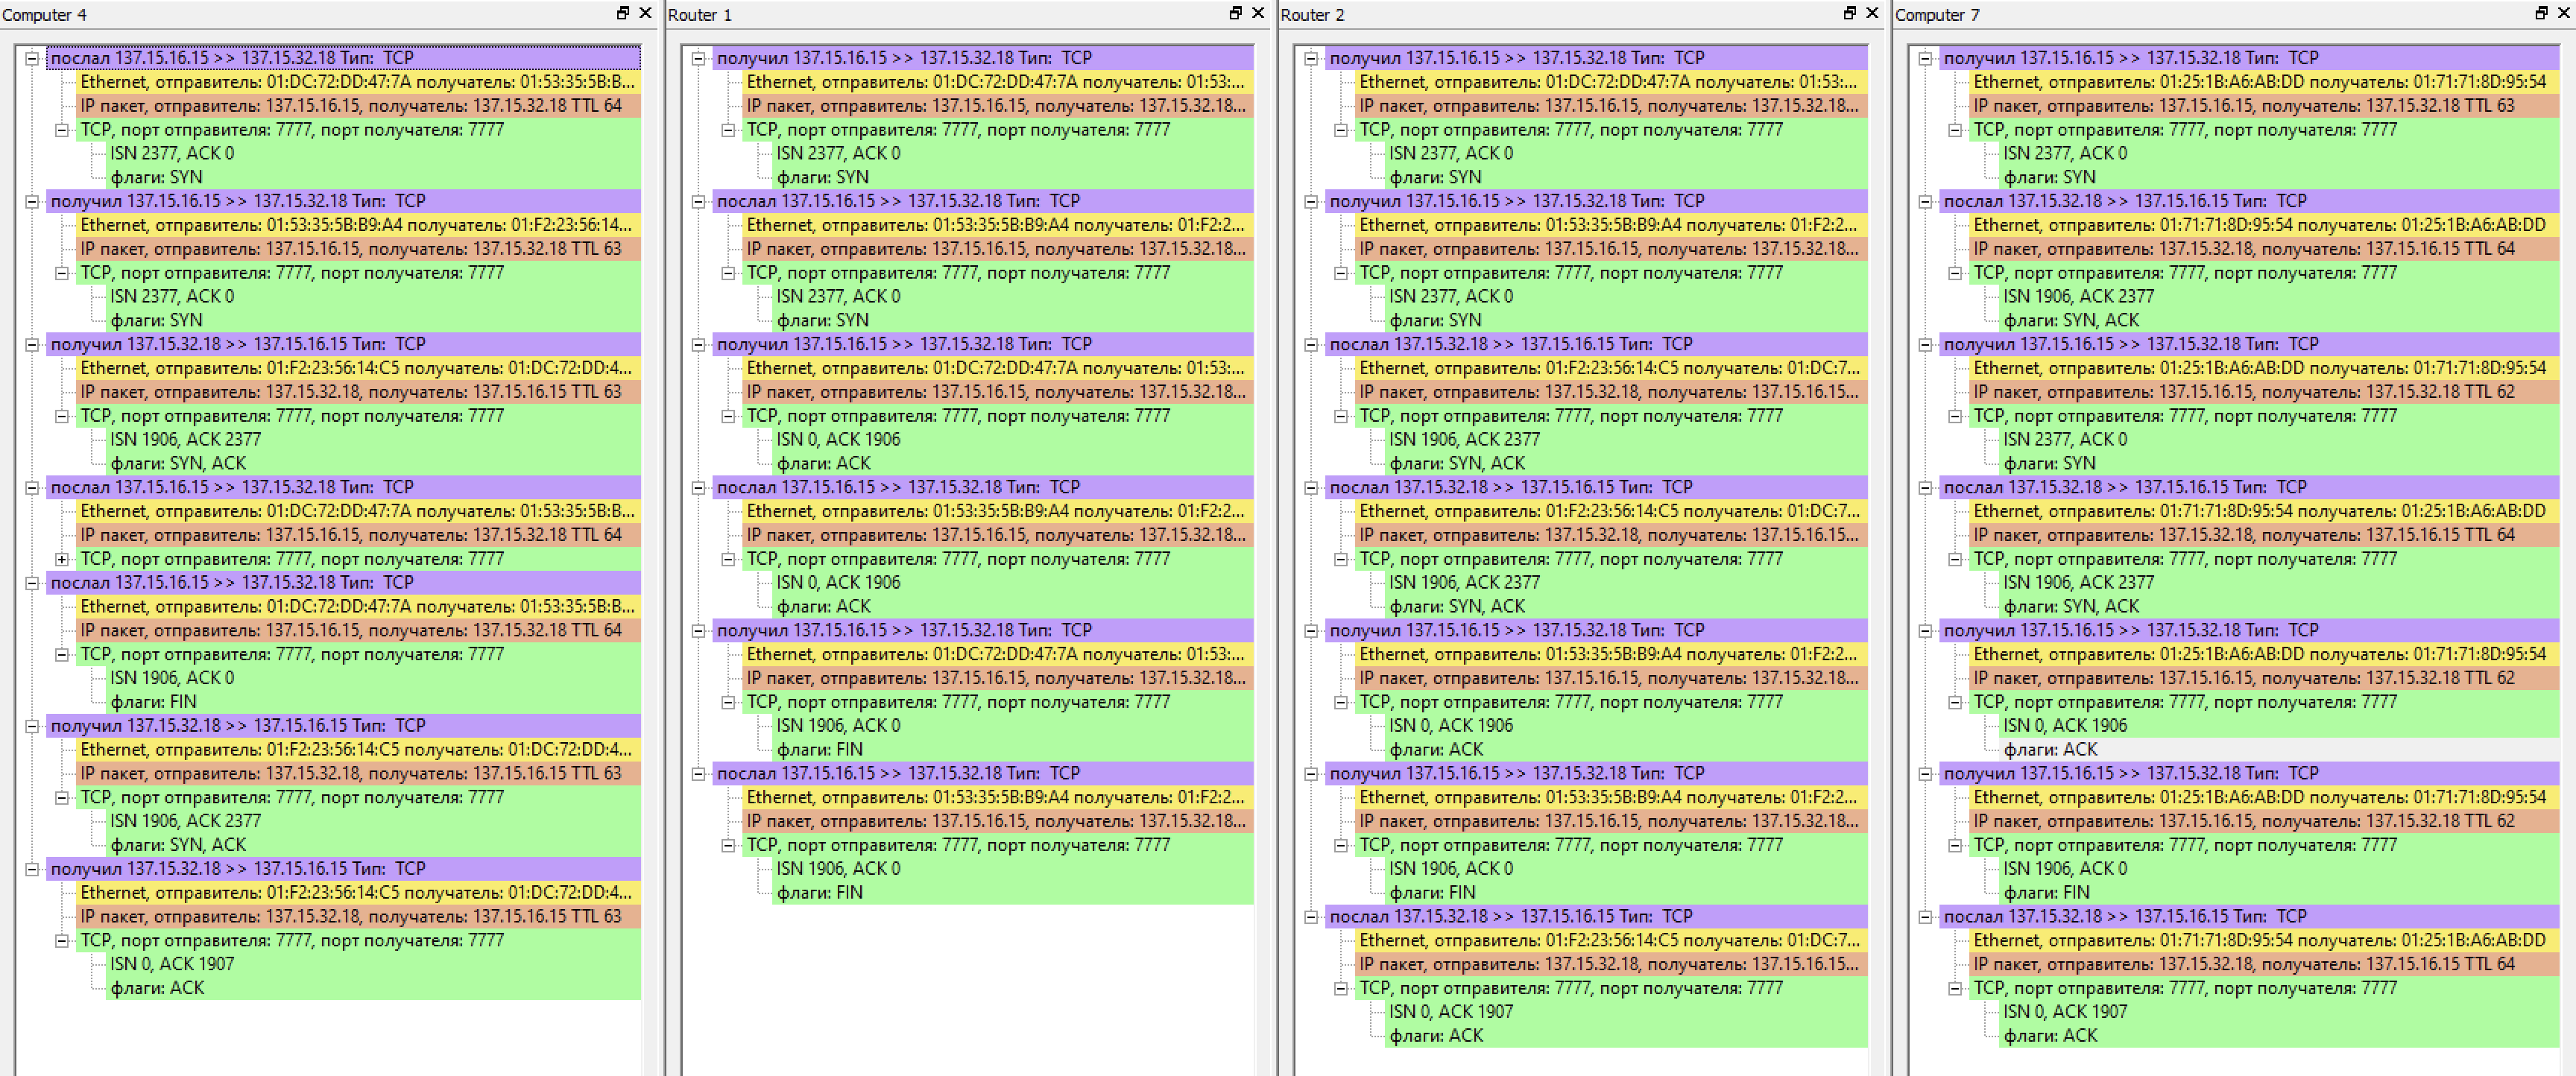
\includegraphics[width=\textwidth]{image/part-2/tcp.png}
    \caption{Отправка TCP пакетов}
\end{figure}
Принцип отправки TCP пакетов аналогичен предыдущему пункту.
\section{ЗАДАНИЕ 3. Сеть тремя маршрутизаторами}
\subsection{Построение сети.}

\begin{figure}[H]
    \centering
    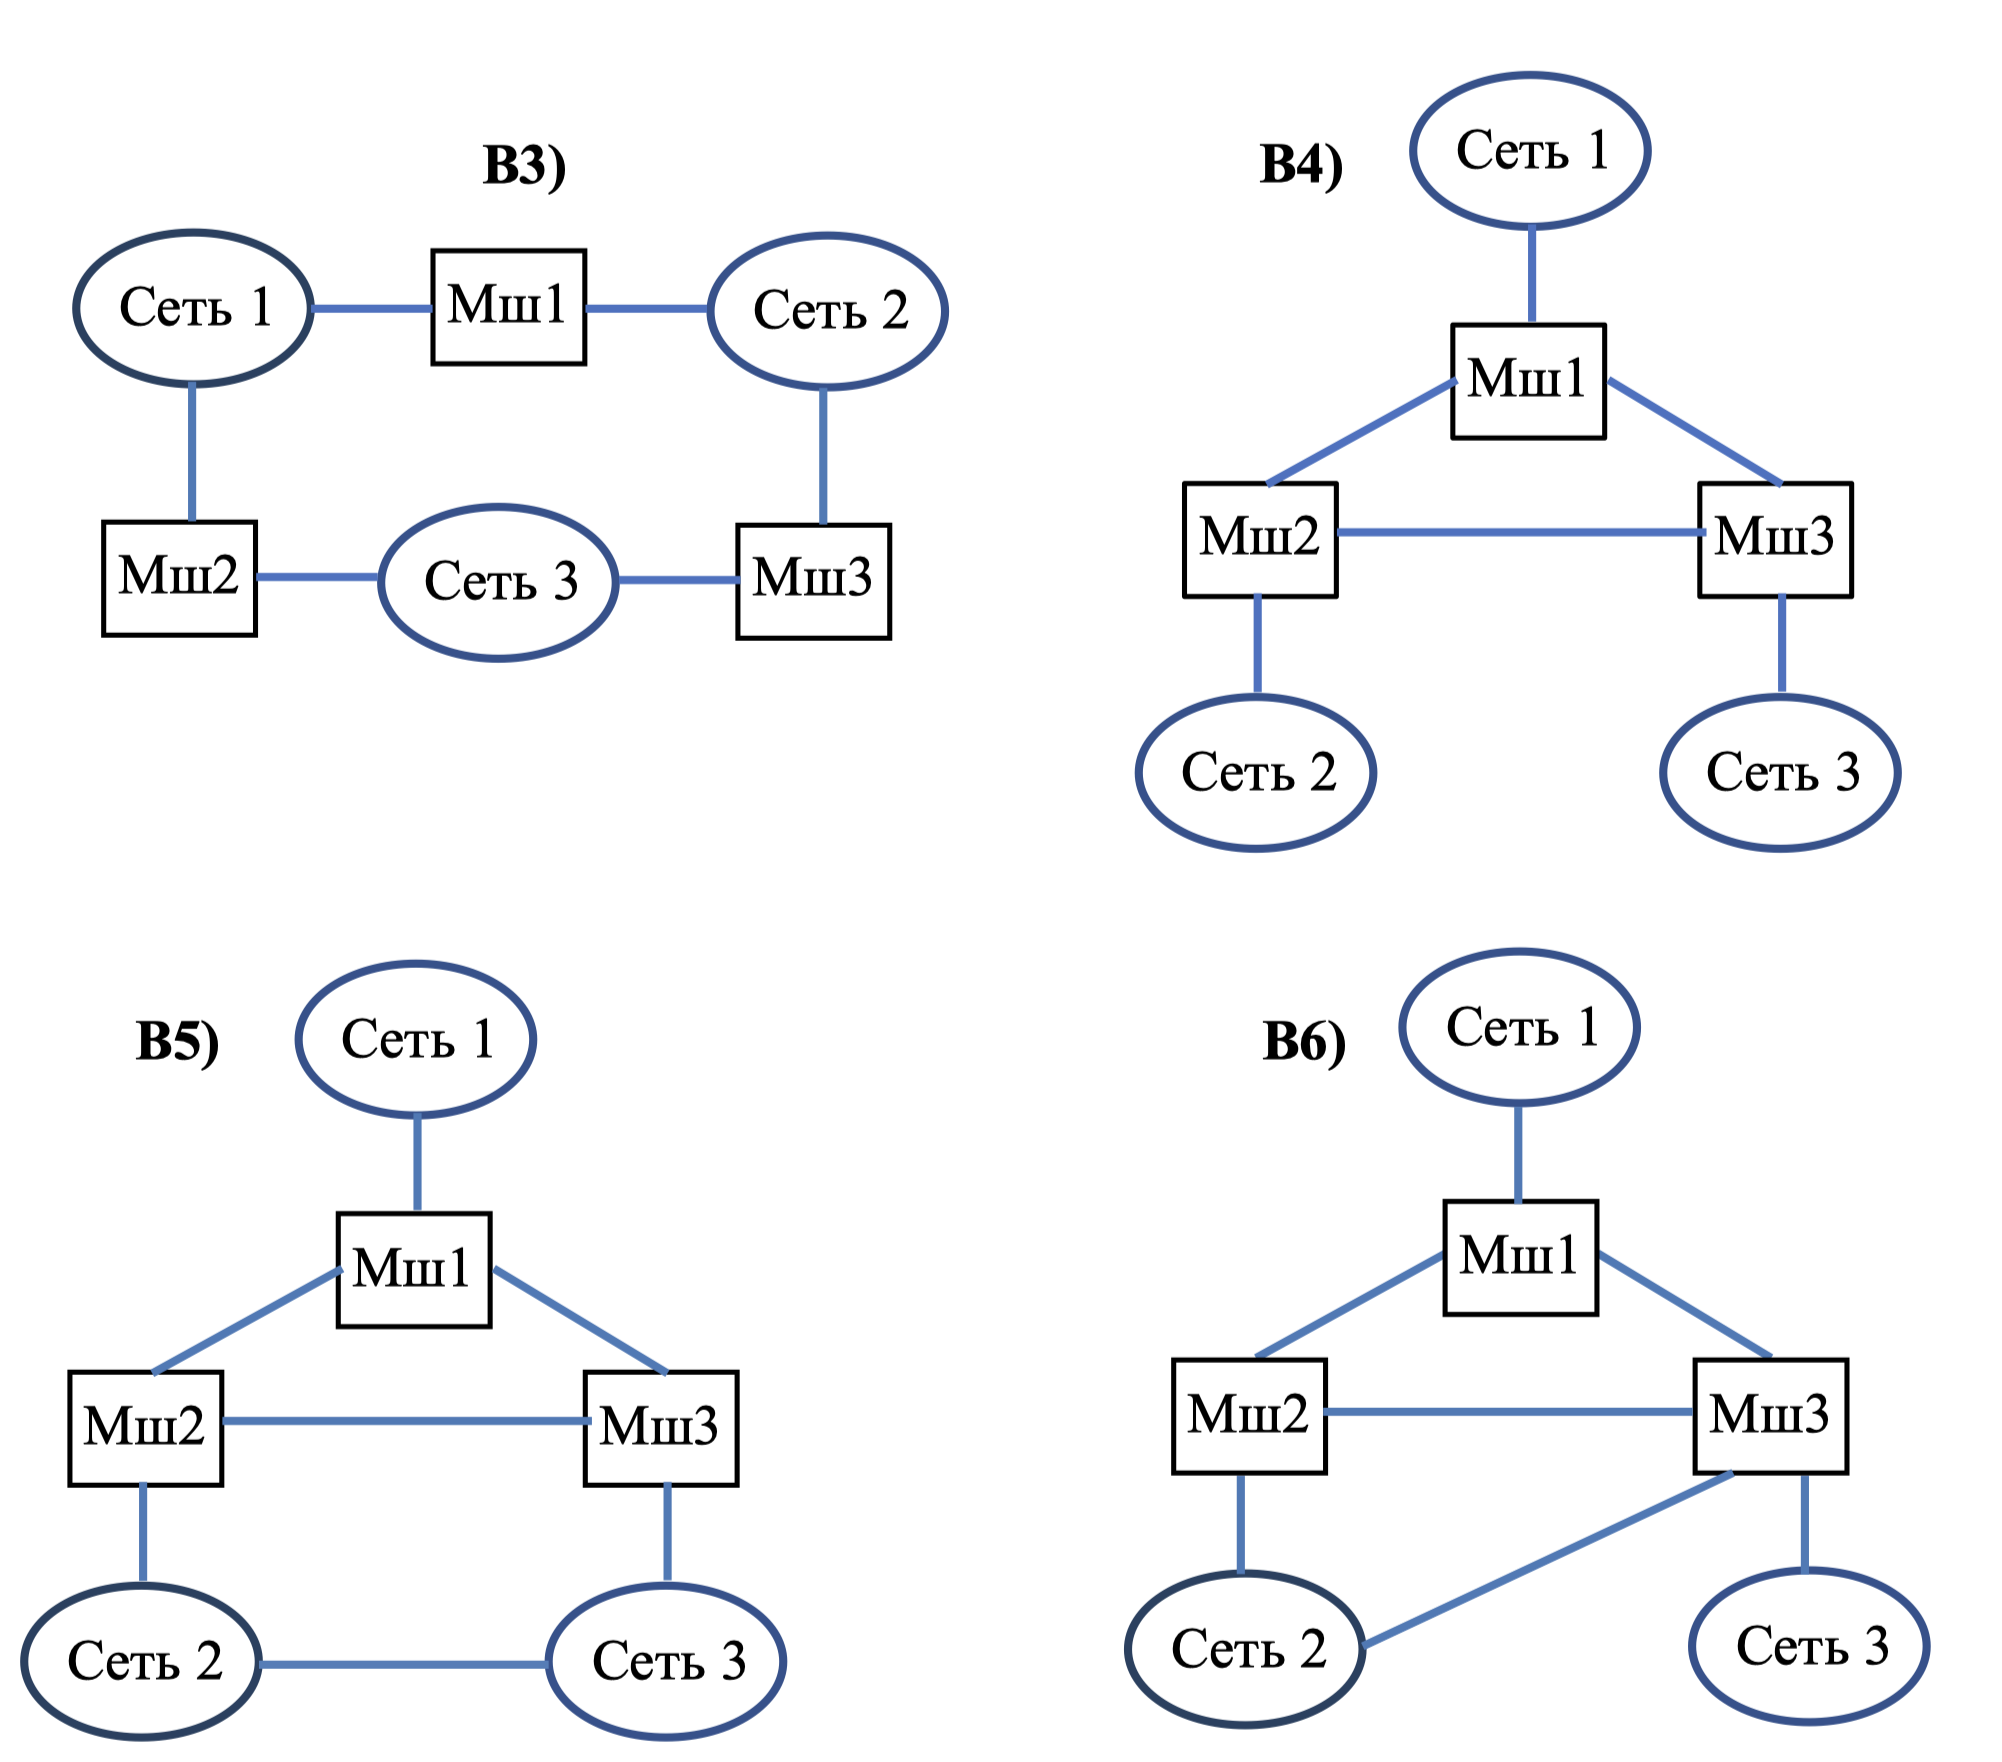
\includegraphics[width=0.5\textwidth]{image/part-3/task3.png}
    \caption{Схемы построения КС с тремя маршрутизаторами}
\end{figure}

\begin{figure}[H]
    \centering
    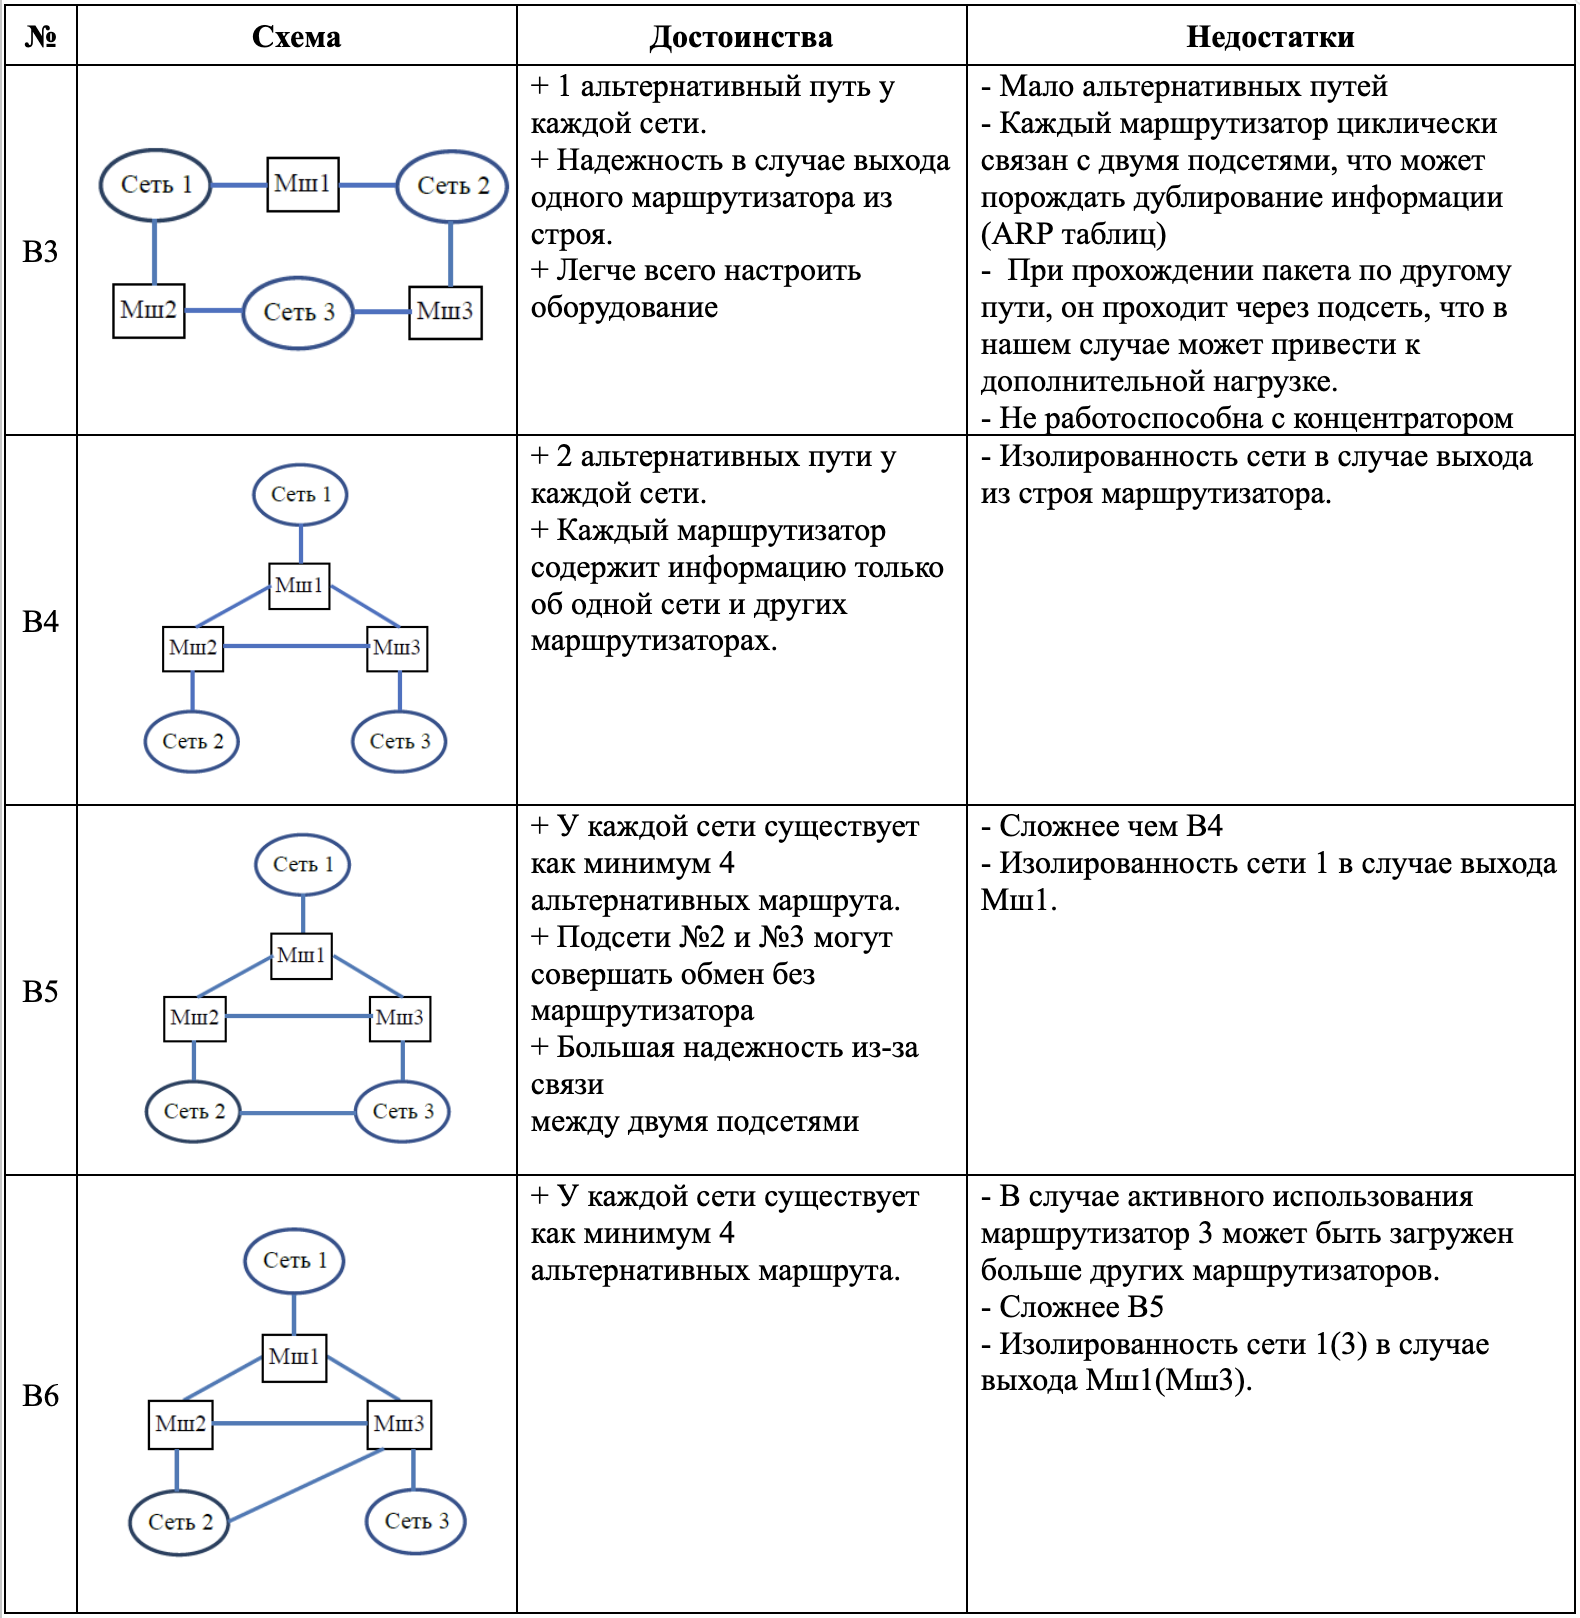
\includegraphics[width=\textwidth]{image/part-3/table.png}
\end{figure}

\subsection{Сеть с тремя маршрутизаторами B5}
\begin{figure}[H]
    \centering
    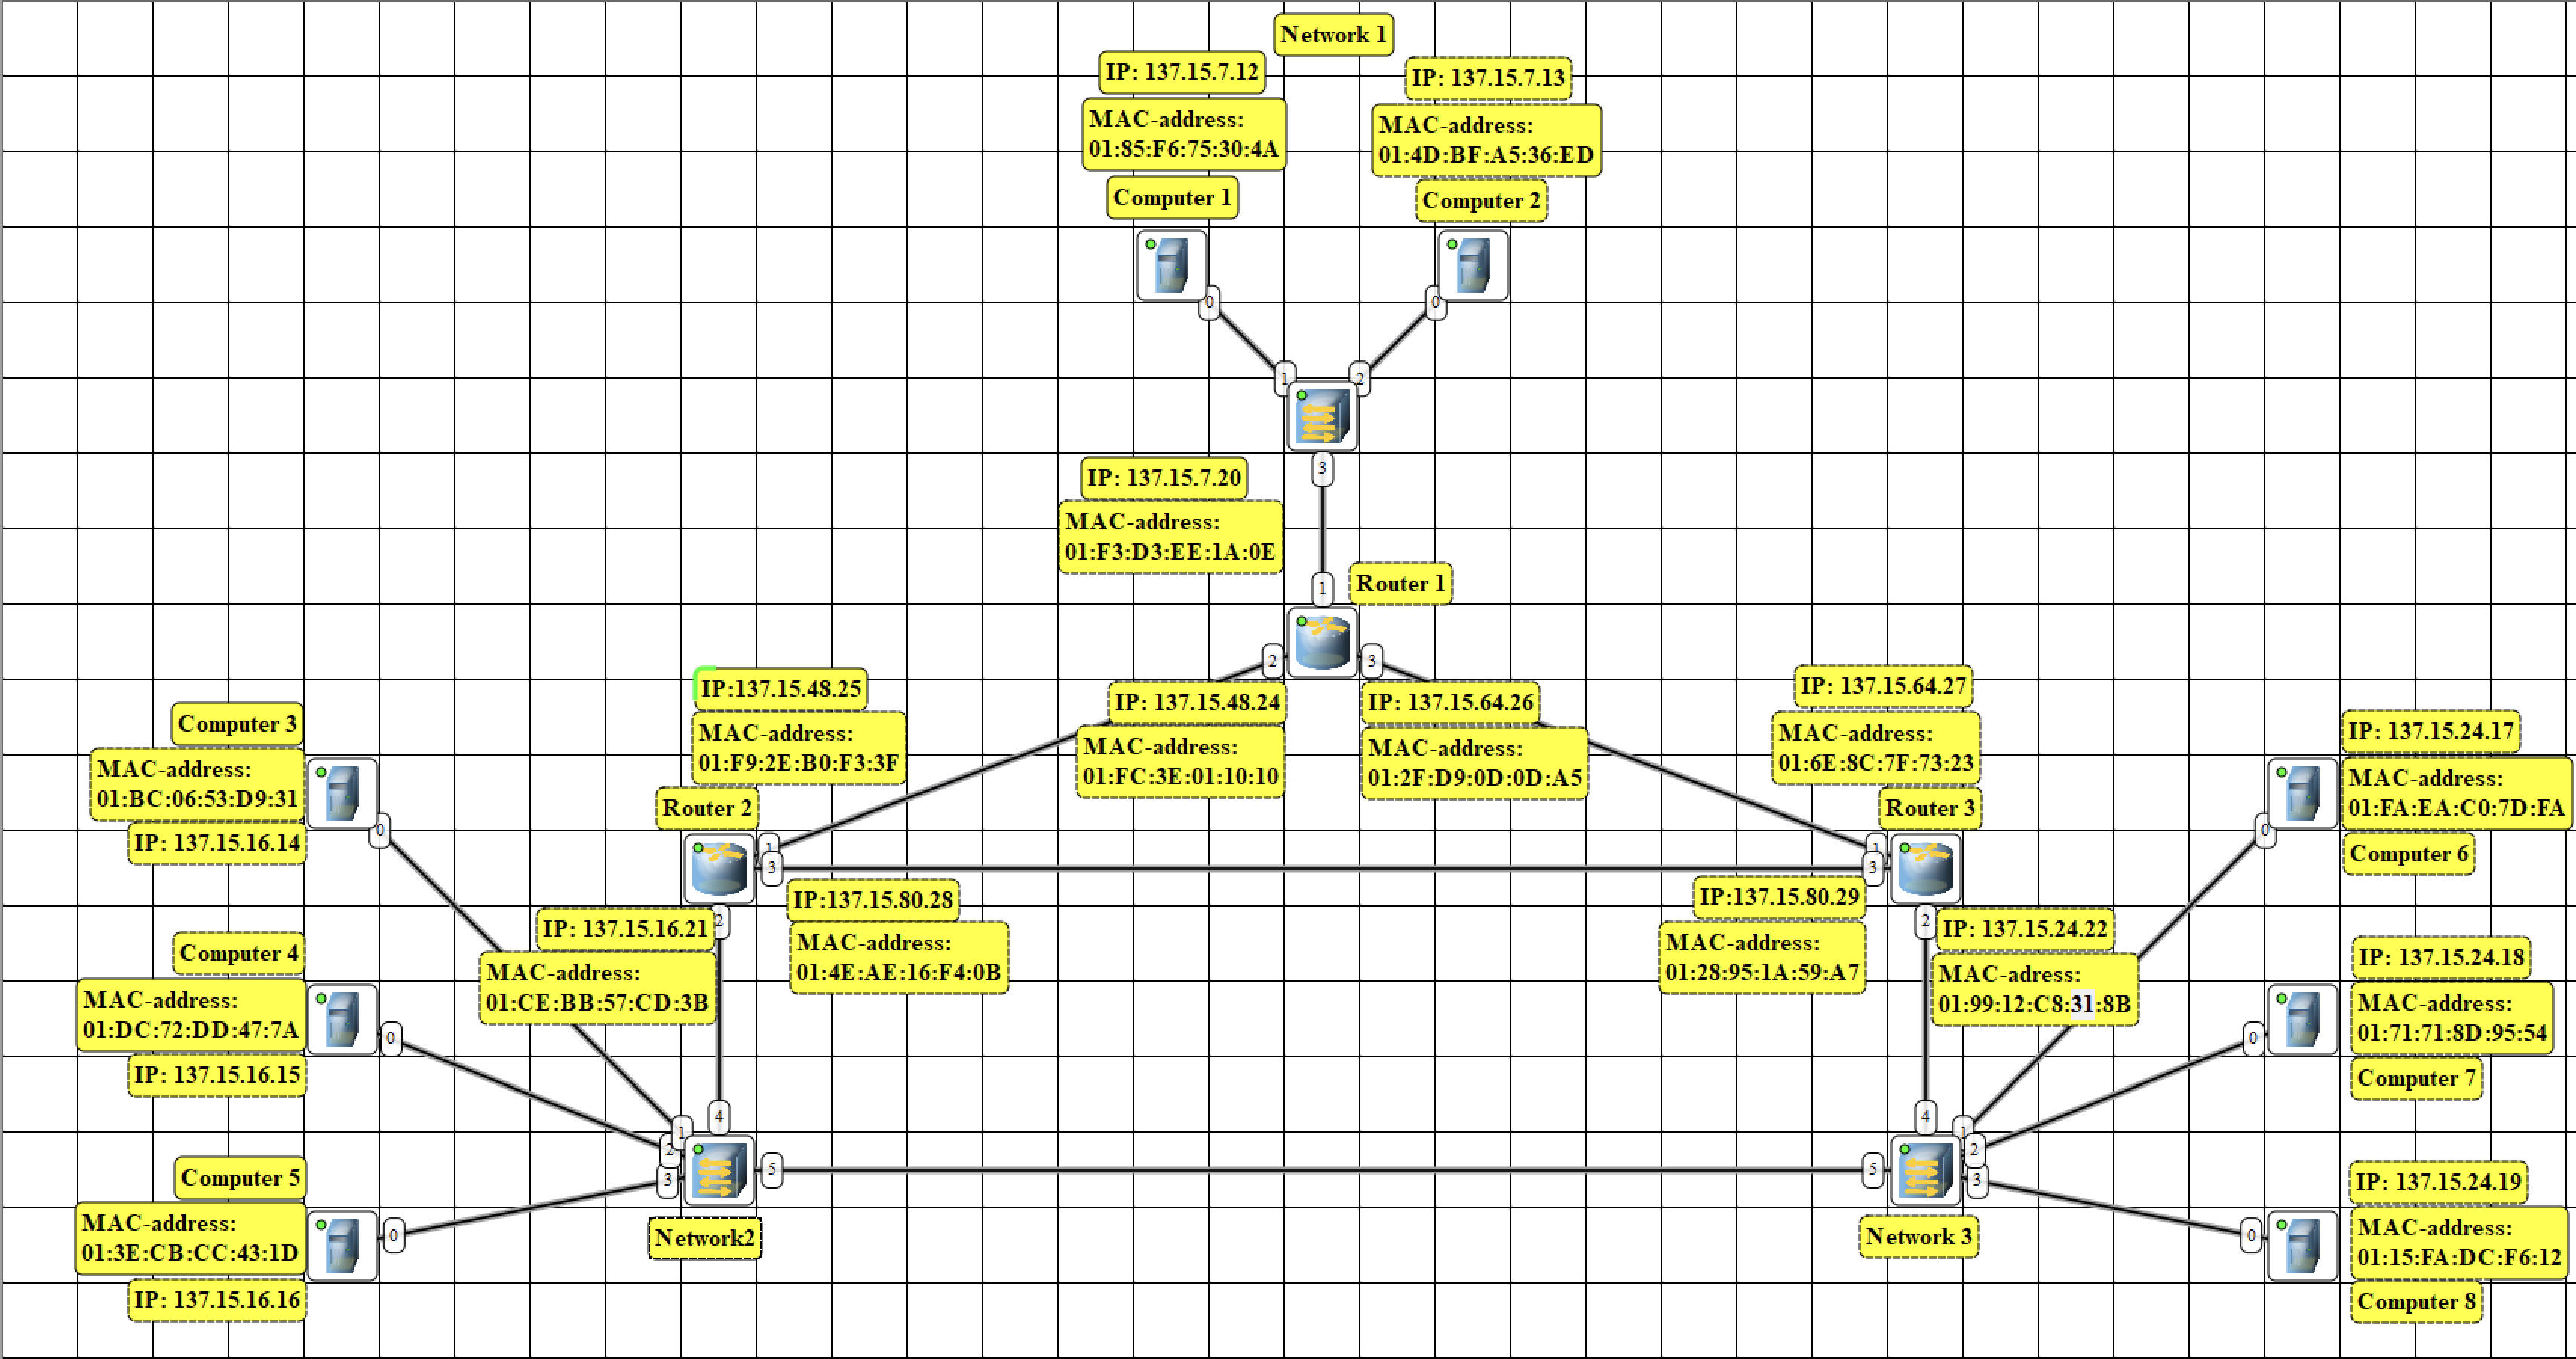
\includegraphics[width=\textwidth]{image/part-3/net3.png}
    \caption{Построенная сеть с тремя маршрутизаторами: В5}
\end{figure}

Преимущество этого варианта в том, что между маршрутизаторами есть подсеть, что упрощает настройку маршрутизации. В отличие от варианта B4, здесь есть соединение между подсетями 2 и 3. Конфигурация была разработана таким образом, что если это соединение присутствует, то обмен пакетами между этими подсетями будет осуществляться через него. Однако если это соединение вдруг исчезнет, нужно будет лишь изменить маску компьютеров (на 22 бита), чтобы запросы шли на шлюзы по умолчанию (Router 2 и Router 3).

В отличие от варианта ВЗ, в данном варианте не происходит дублирования пакета из-за концентратора, так как он связан только с одним маршрутизатором.

Ниже представлены таблицы маршрутизации компьютеров и маршрутизаторов.

\begin{figure}[H]
    \centering
    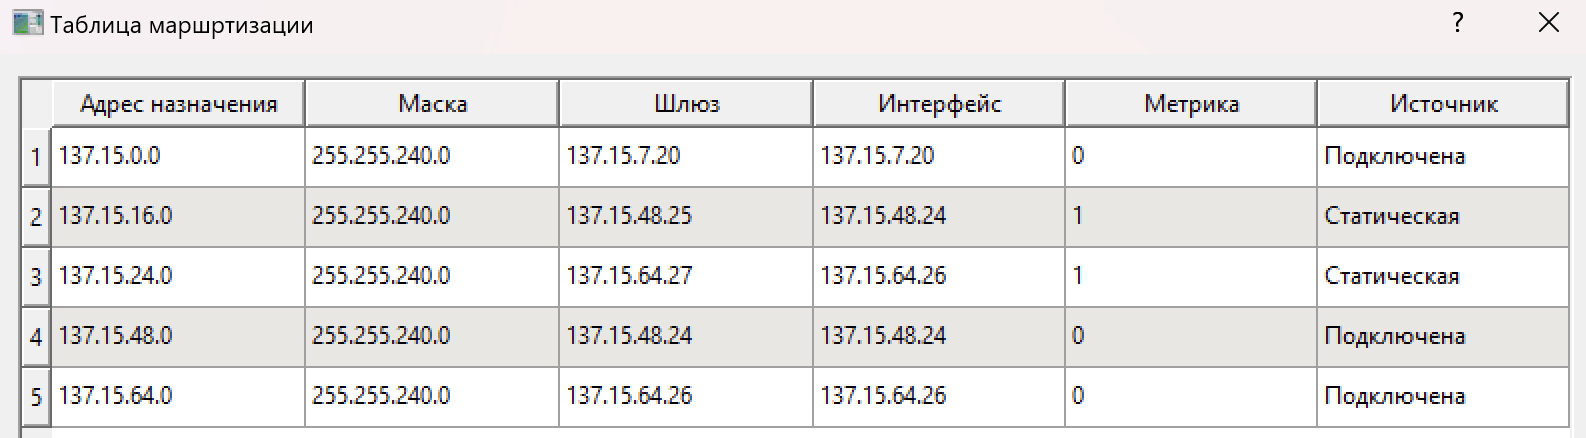
\includegraphics[width=\textwidth]{image/part-3/router1.png}
    \caption{Таблица маршрутизации маршрутизатора 1}
\end{figure}

\begin{figure}[H]
    \centering
    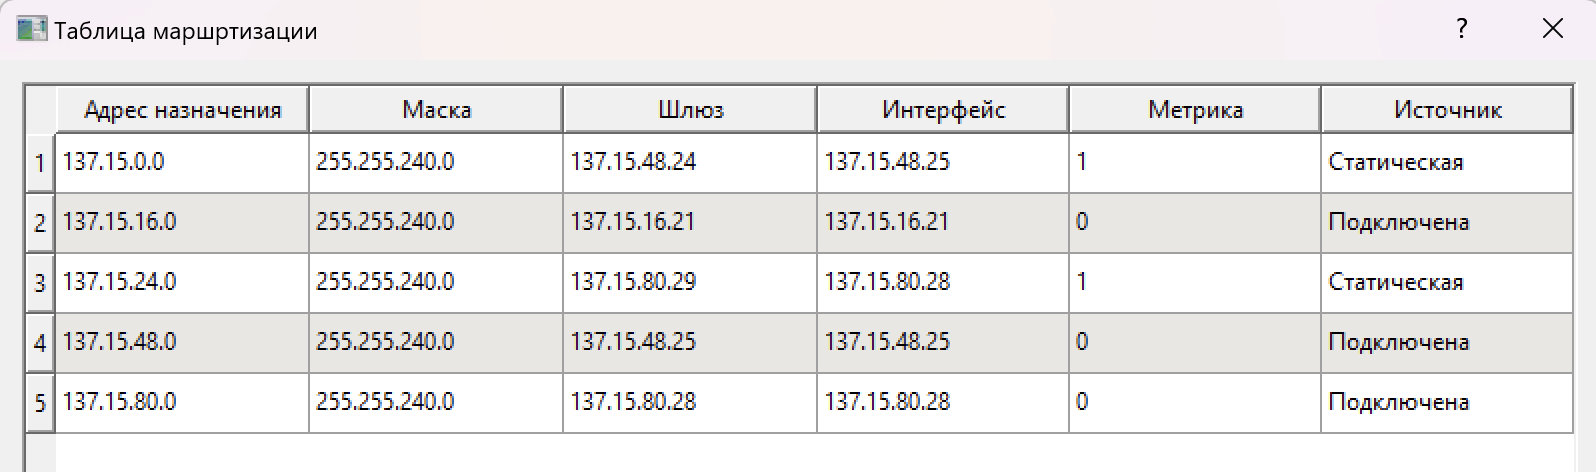
\includegraphics[width=\textwidth]{image/part-3/router2.png}
    \caption{Таблица маршрутизации маршрутизатора 2}
\end{figure}

\begin{figure}[H]
    \centering
    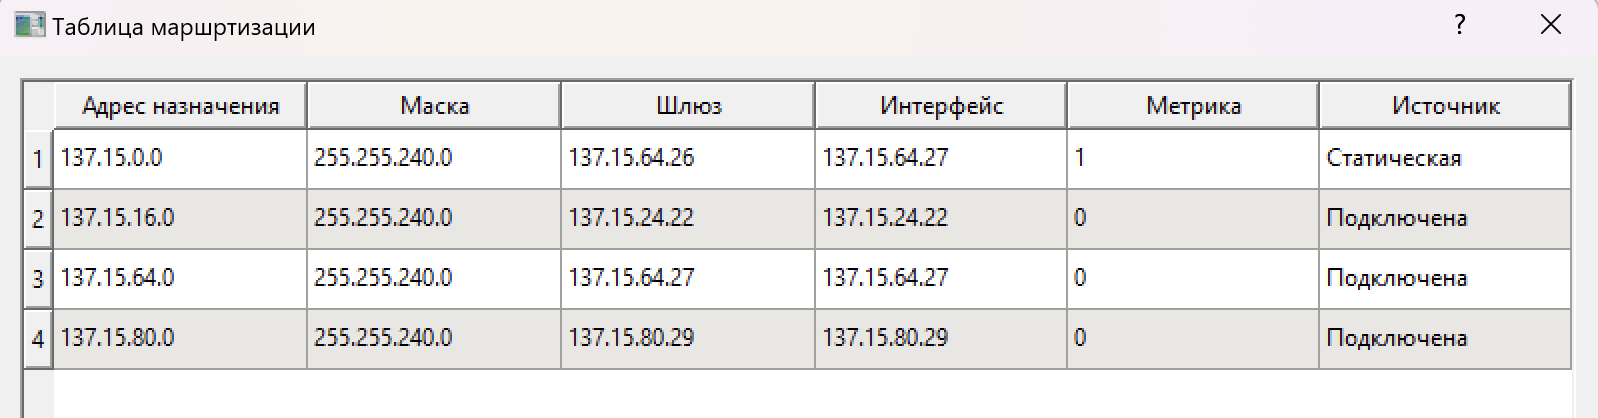
\includegraphics[width=\textwidth]{image/part-3/router3.png}
    \caption{Таблица маршрутизации маршрутизатора 3}
\end{figure}

\begin{figure}[H]
    \centering
    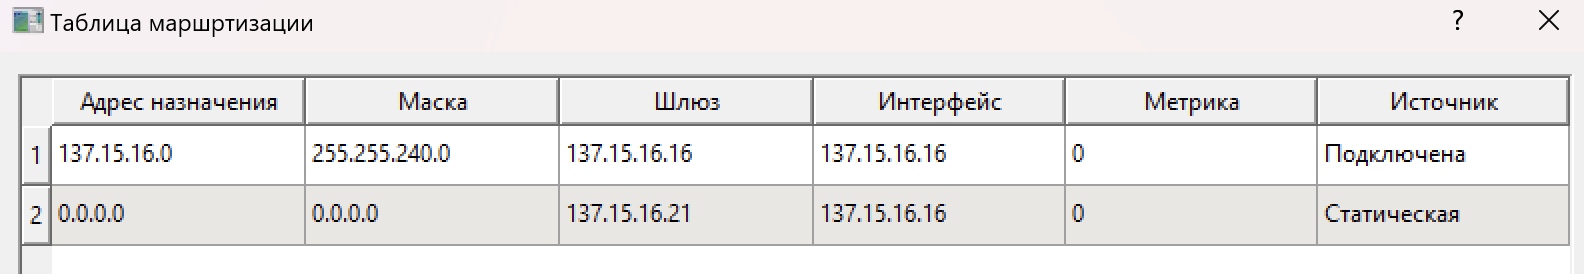
\includegraphics[width=\textwidth]{image/part-3/computer5.png}
    \caption{Таблица маршрутизации компьютера 5}
\end{figure}

\begin{figure}[H]
    \centering
    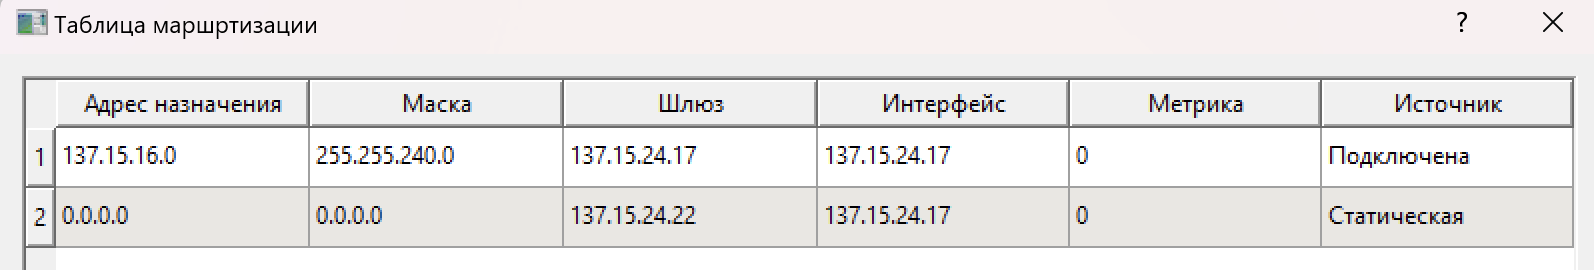
\includegraphics[width=\textwidth]{image/part-3/computer6.png}
    \caption{Таблица маршрутизации компьютера 6}
\end{figure}

\begin{figure}[H]
    \centering
    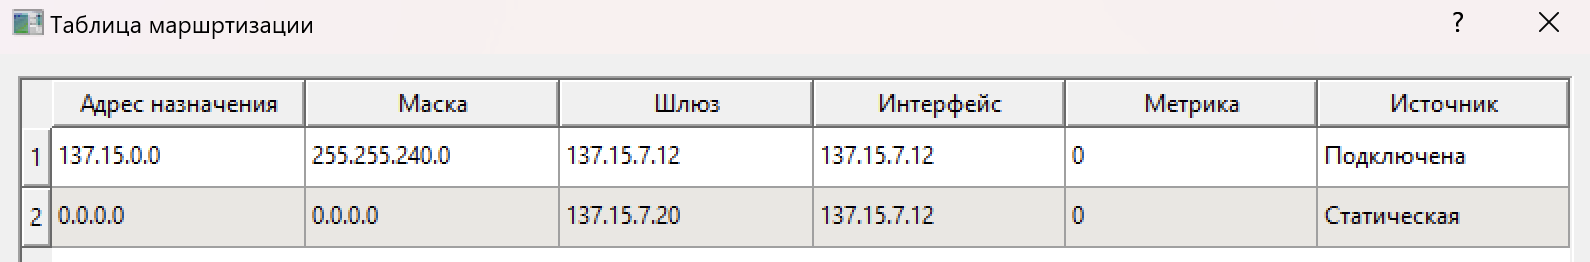
\includegraphics[width=\textwidth]{image/part-3/computer1.png}
    \caption{Таблица маршрутизации компьютера 1}
\end{figure}
\subsection{Тестирование сети (отправка пакетов).}
\subsubsection{UDP}
\begin{figure}[H]
    \centering
    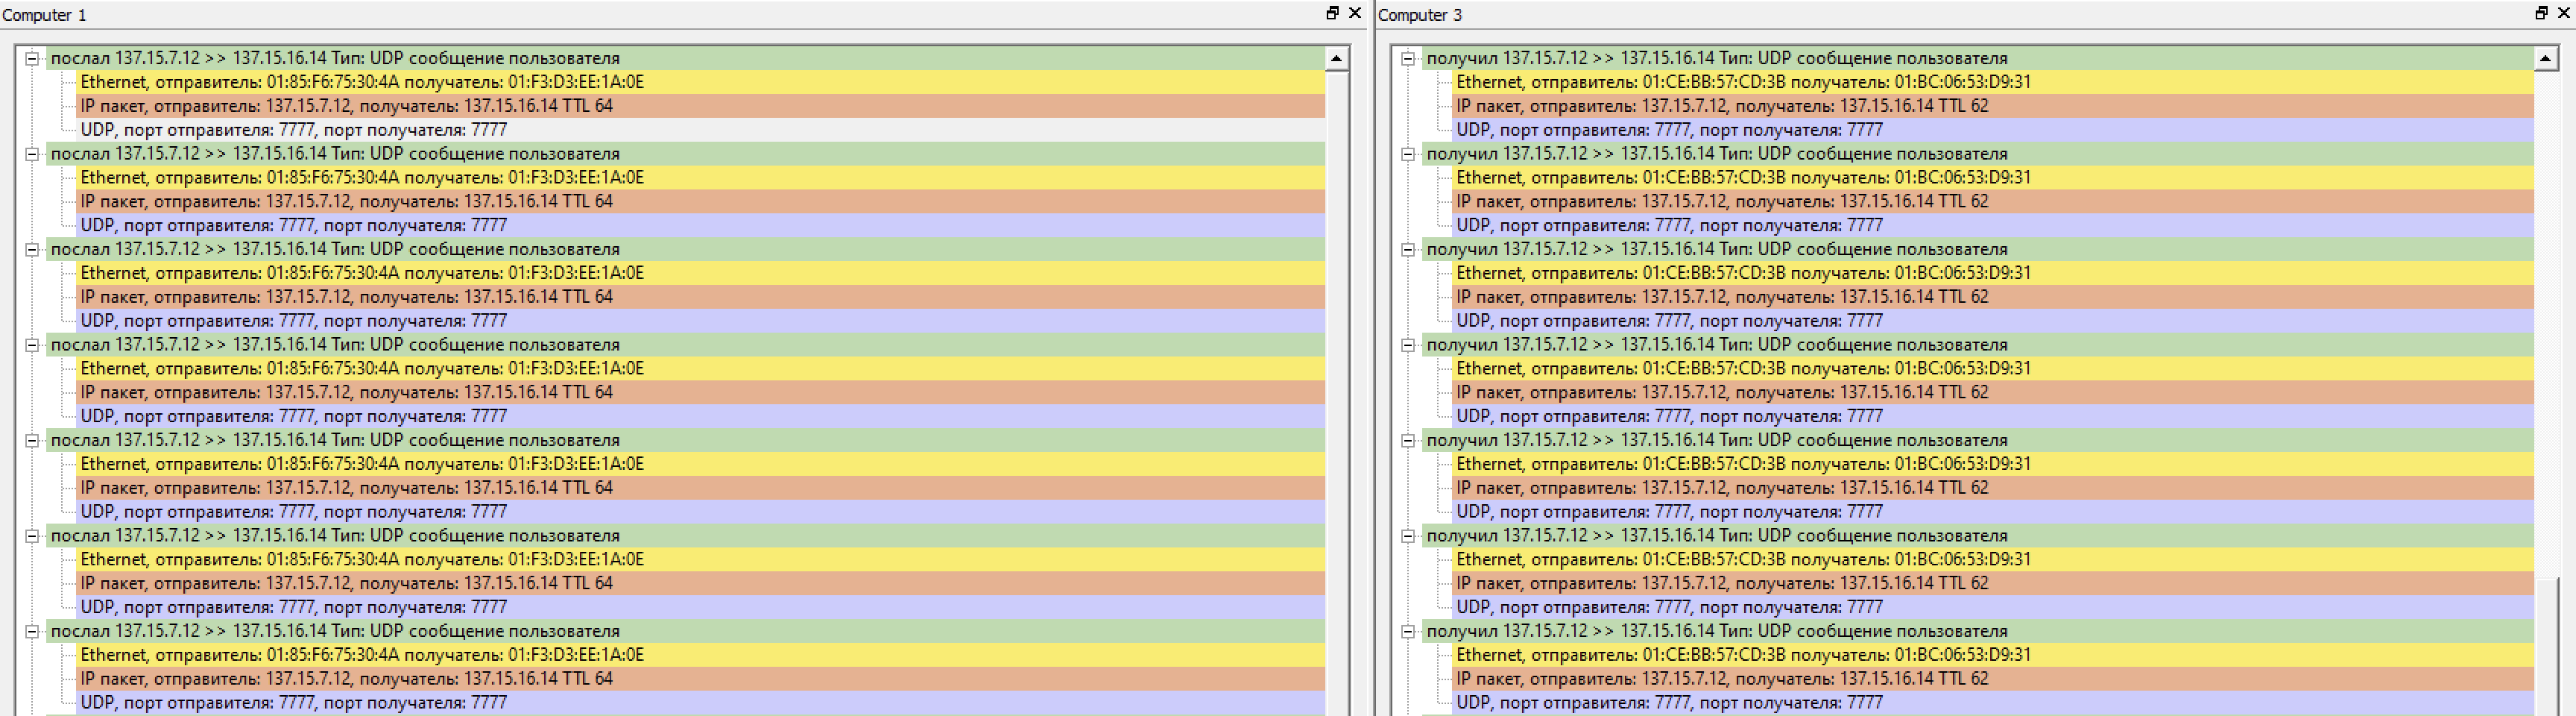
\includegraphics[width=\textwidth]{image/part-3/udp.png}
    \caption{Отправка UDP пакетов}
\end{figure}
\subsubsection{TCP}
\begin{figure}[H]
    \centering
    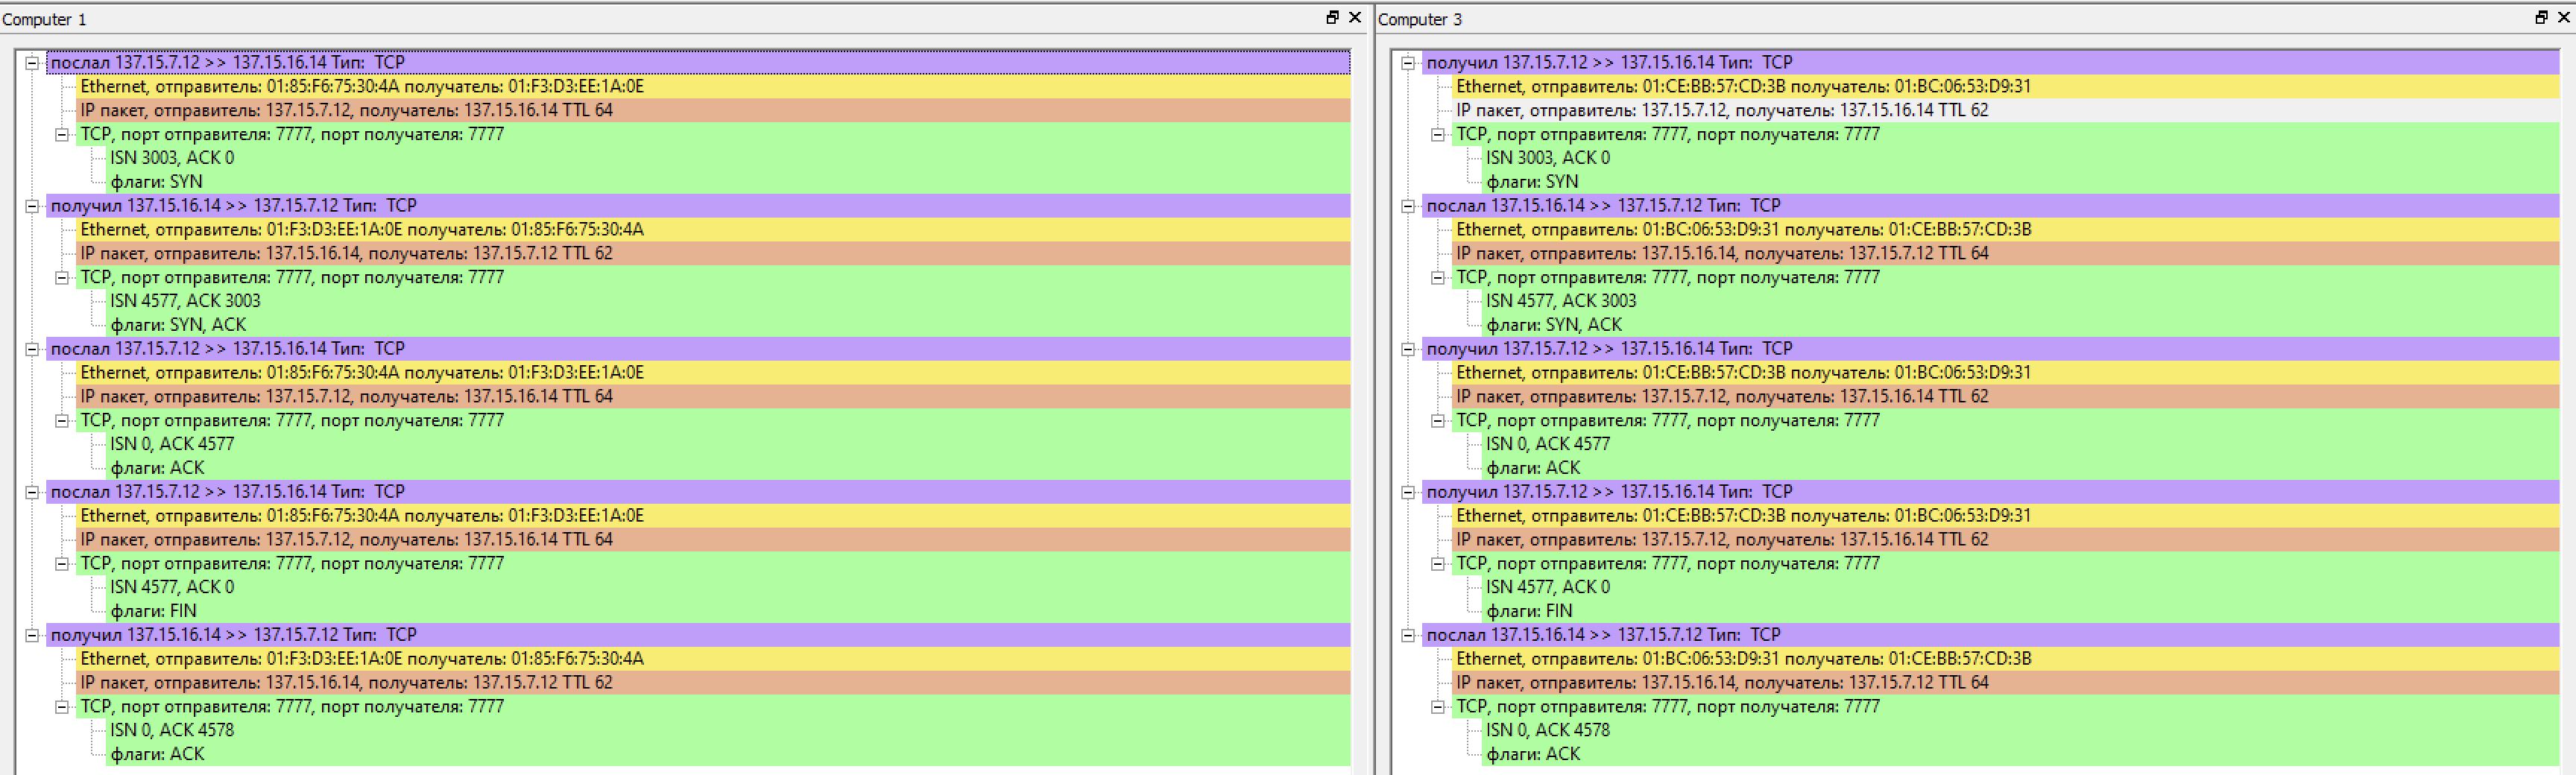
\includegraphics[width=\textwidth]{image/part-3/tcp.png}
    \caption{Отправка TCP пакетов}
\end{figure}

Журналы ТСР и UDP аналогичны предыдущим пунктам.

\section{Настройка динамической маршрутизации по протоколу RIP.}

Динамическая маршрутизация - это процесс, при котором маршруты в сети определяются автоматически с помощью протоколов маршрутизации. 

В случае с RIP расстояние определяется количеством промежуточных маршрутизаторов. Протокол извлекает информацию о новых сетях из сообщений, полученных от соседних маршрутизаторов. Маршрутизаторы обмениваются сообщениями каждые 30 секунд, и если в течение 180 секунд от маршрутизатора не поступило ни одного сообщения, то он считается вышедшим из строя.


\begin{figure}[H]
    \centering
    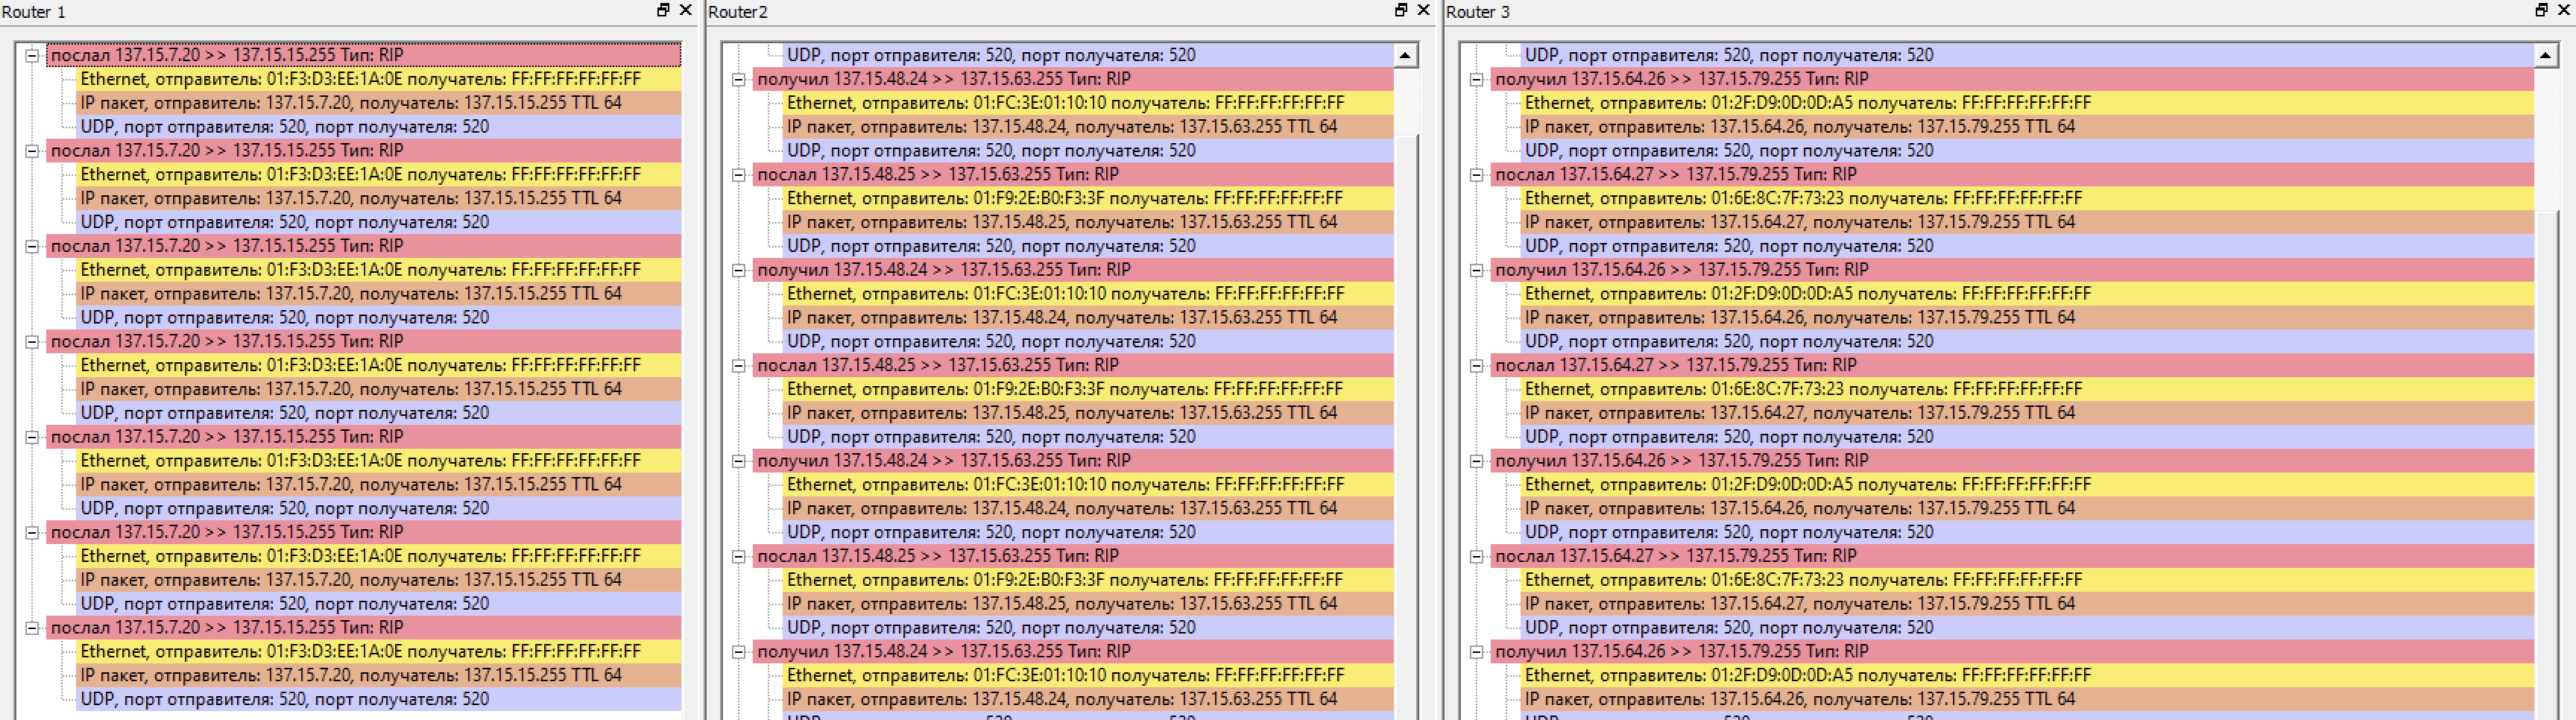
\includegraphics[width=\textwidth]{image/part-4/RIP.png}
    \caption{Работа RIP}
\end{figure}
Как можно заметить, МАС адрес получателя является широковещательным.
Рассылка происходит по всем интерфейсам маршрутизатора.
Получатель -- любое устройство, которое находятся в искомой подсети.

Этапы работы RIP:
\begin{enumerate}
    \item Создание минимальной таблицы. В таблице содержатся только непосредственно подсоединенные сети.
    \item Рассылка минимальной таблицы соседям.
    \item Получение RIP-сообщений от соседей.  Увеличивает каждое поле метрики на 1 и если информация о маршруте лучше или это новый пункт назначения, то обновляет таблицу маршрутизации.
    \item Рассылка новой таблицы соседям. 
    \item Повторение шагов 3-4.
\end{enumerate}

\begin{figure}[H]
    \centering
    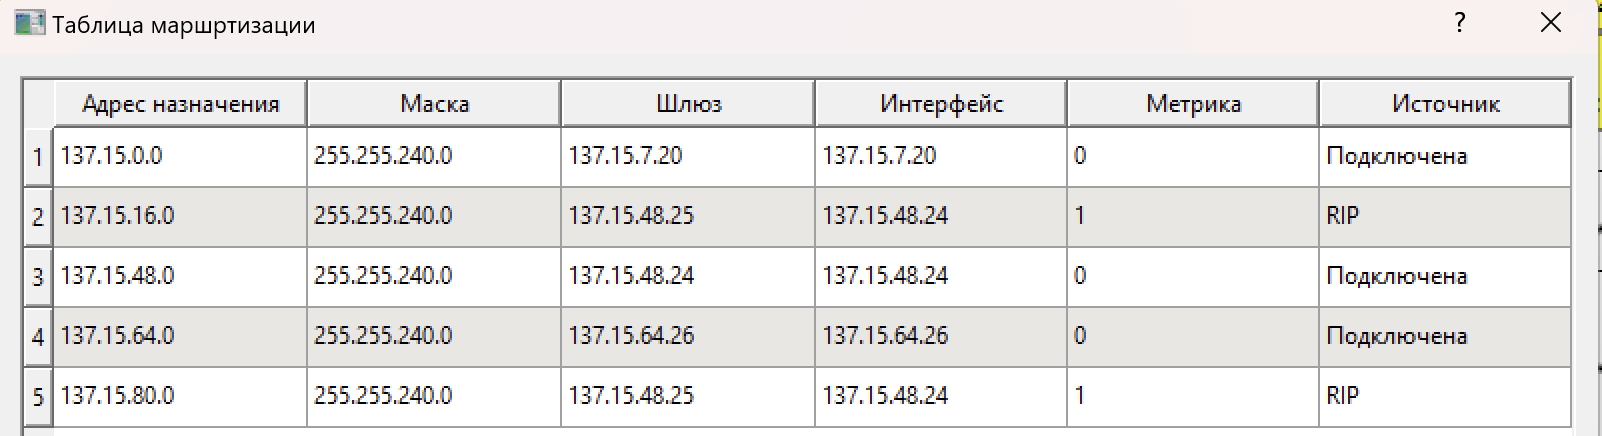
\includegraphics[width=\textwidth]{image/part-4/router1.png}
    \caption{Таблица маршрутизации маршрутизатора 1}
\end{figure}
\begin{figure}[H]
    \centering
    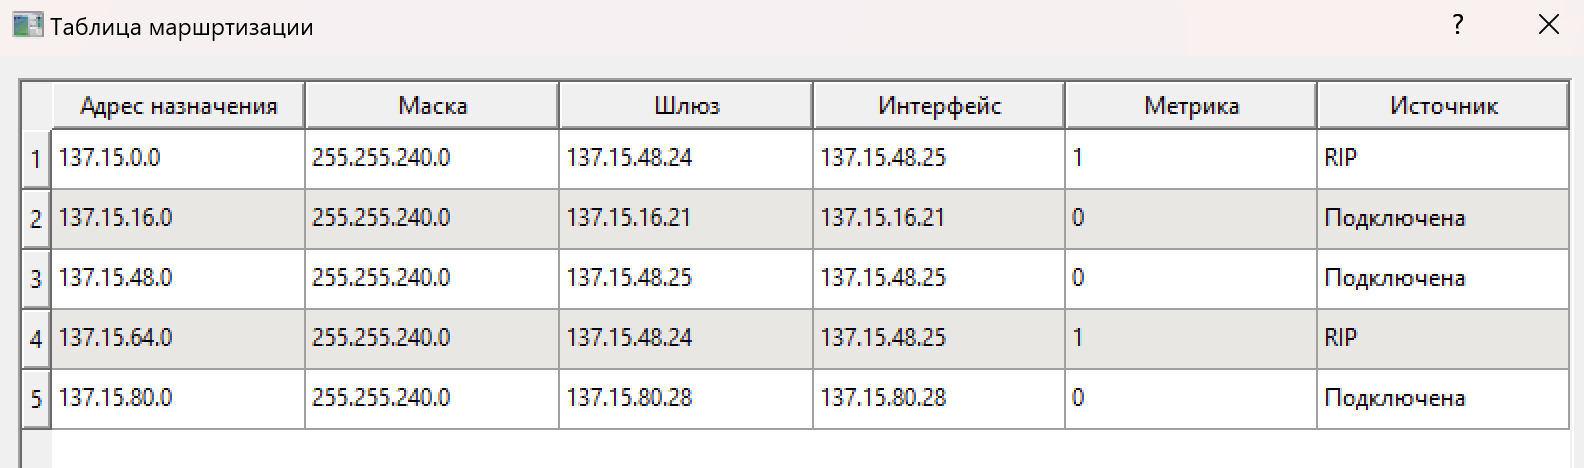
\includegraphics[width=\textwidth]{image/part-4/router2.png}
    \caption{Таблица маршрутизации маршрутизатора 2}
\end{figure}
\begin{figure}[H]
    \centering
    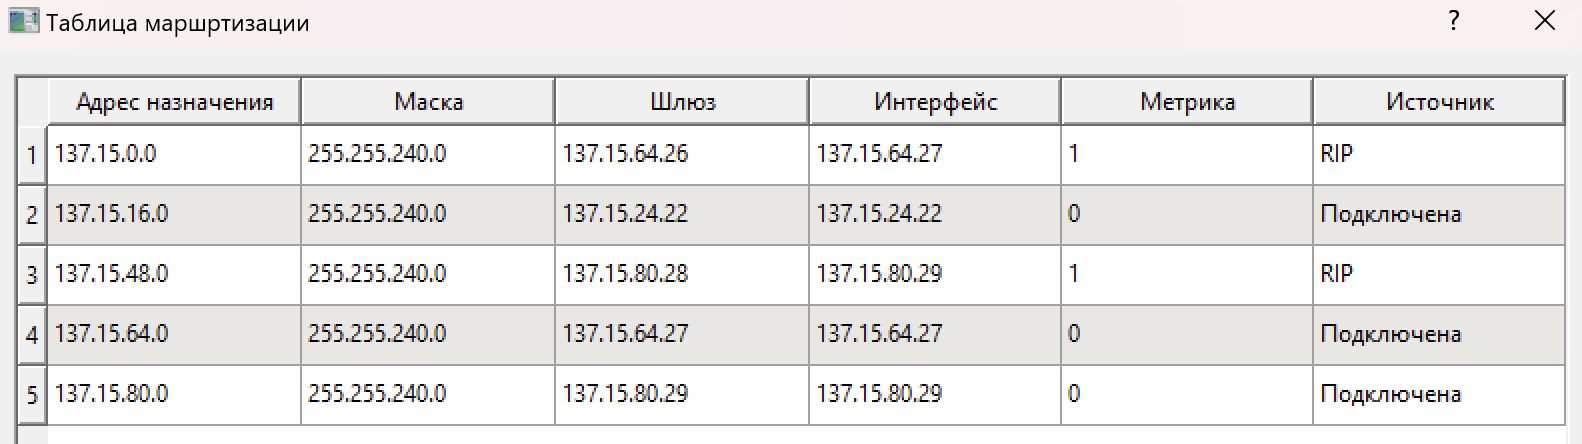
\includegraphics[width=\textwidth]{image/part-4/router3.png}
    \caption{Таблица маршрутизации маршрутизатора 3}
\end{figure}

В таблице маршрутизации записи указаны верно. Кроме того, в отличие от
заданных статических записей, протокол указал подсети между
маршрутизаторами.

\begin{figure}[H]
    \centering
    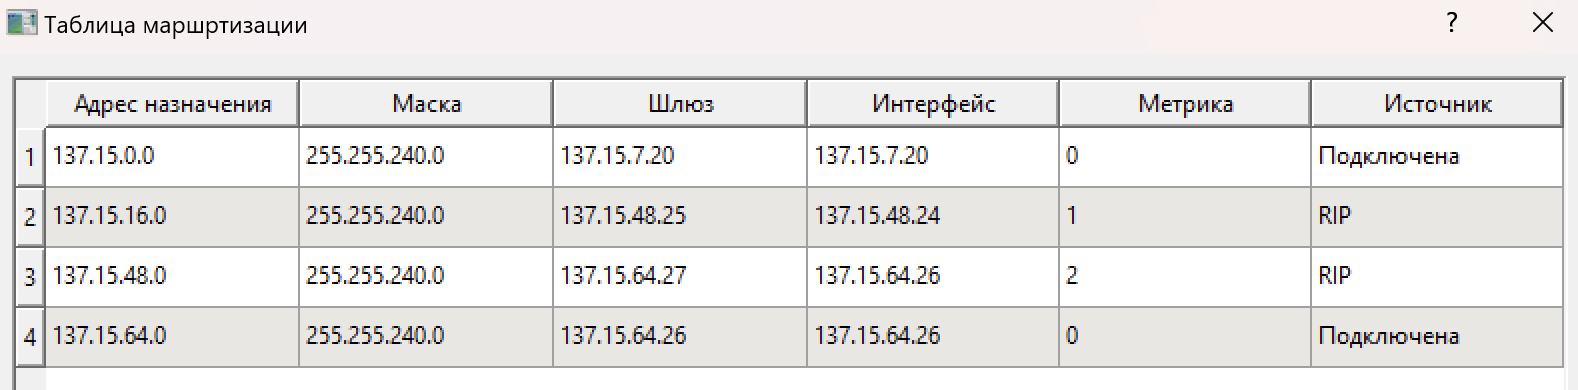
\includegraphics[width=\textwidth]{image/part-4/router1-after.png}
    \caption{Таблица маршрутизации маршрутизатора 1 после удаления М2}
\end{figure}

После удаления М2 из таблицы маршрутизации М1, пропала запись о подсети 137.15.80.0, которая была связана с М2.

Таким образом, если удалить маршрутизатор из сети, то из других
маршрутизаторов со временем удалятся соответствующие записи.

\section{Настройка автоматического получения сетевых настроек по протоколу DHCP.}
\begin{figure}
    \centering
    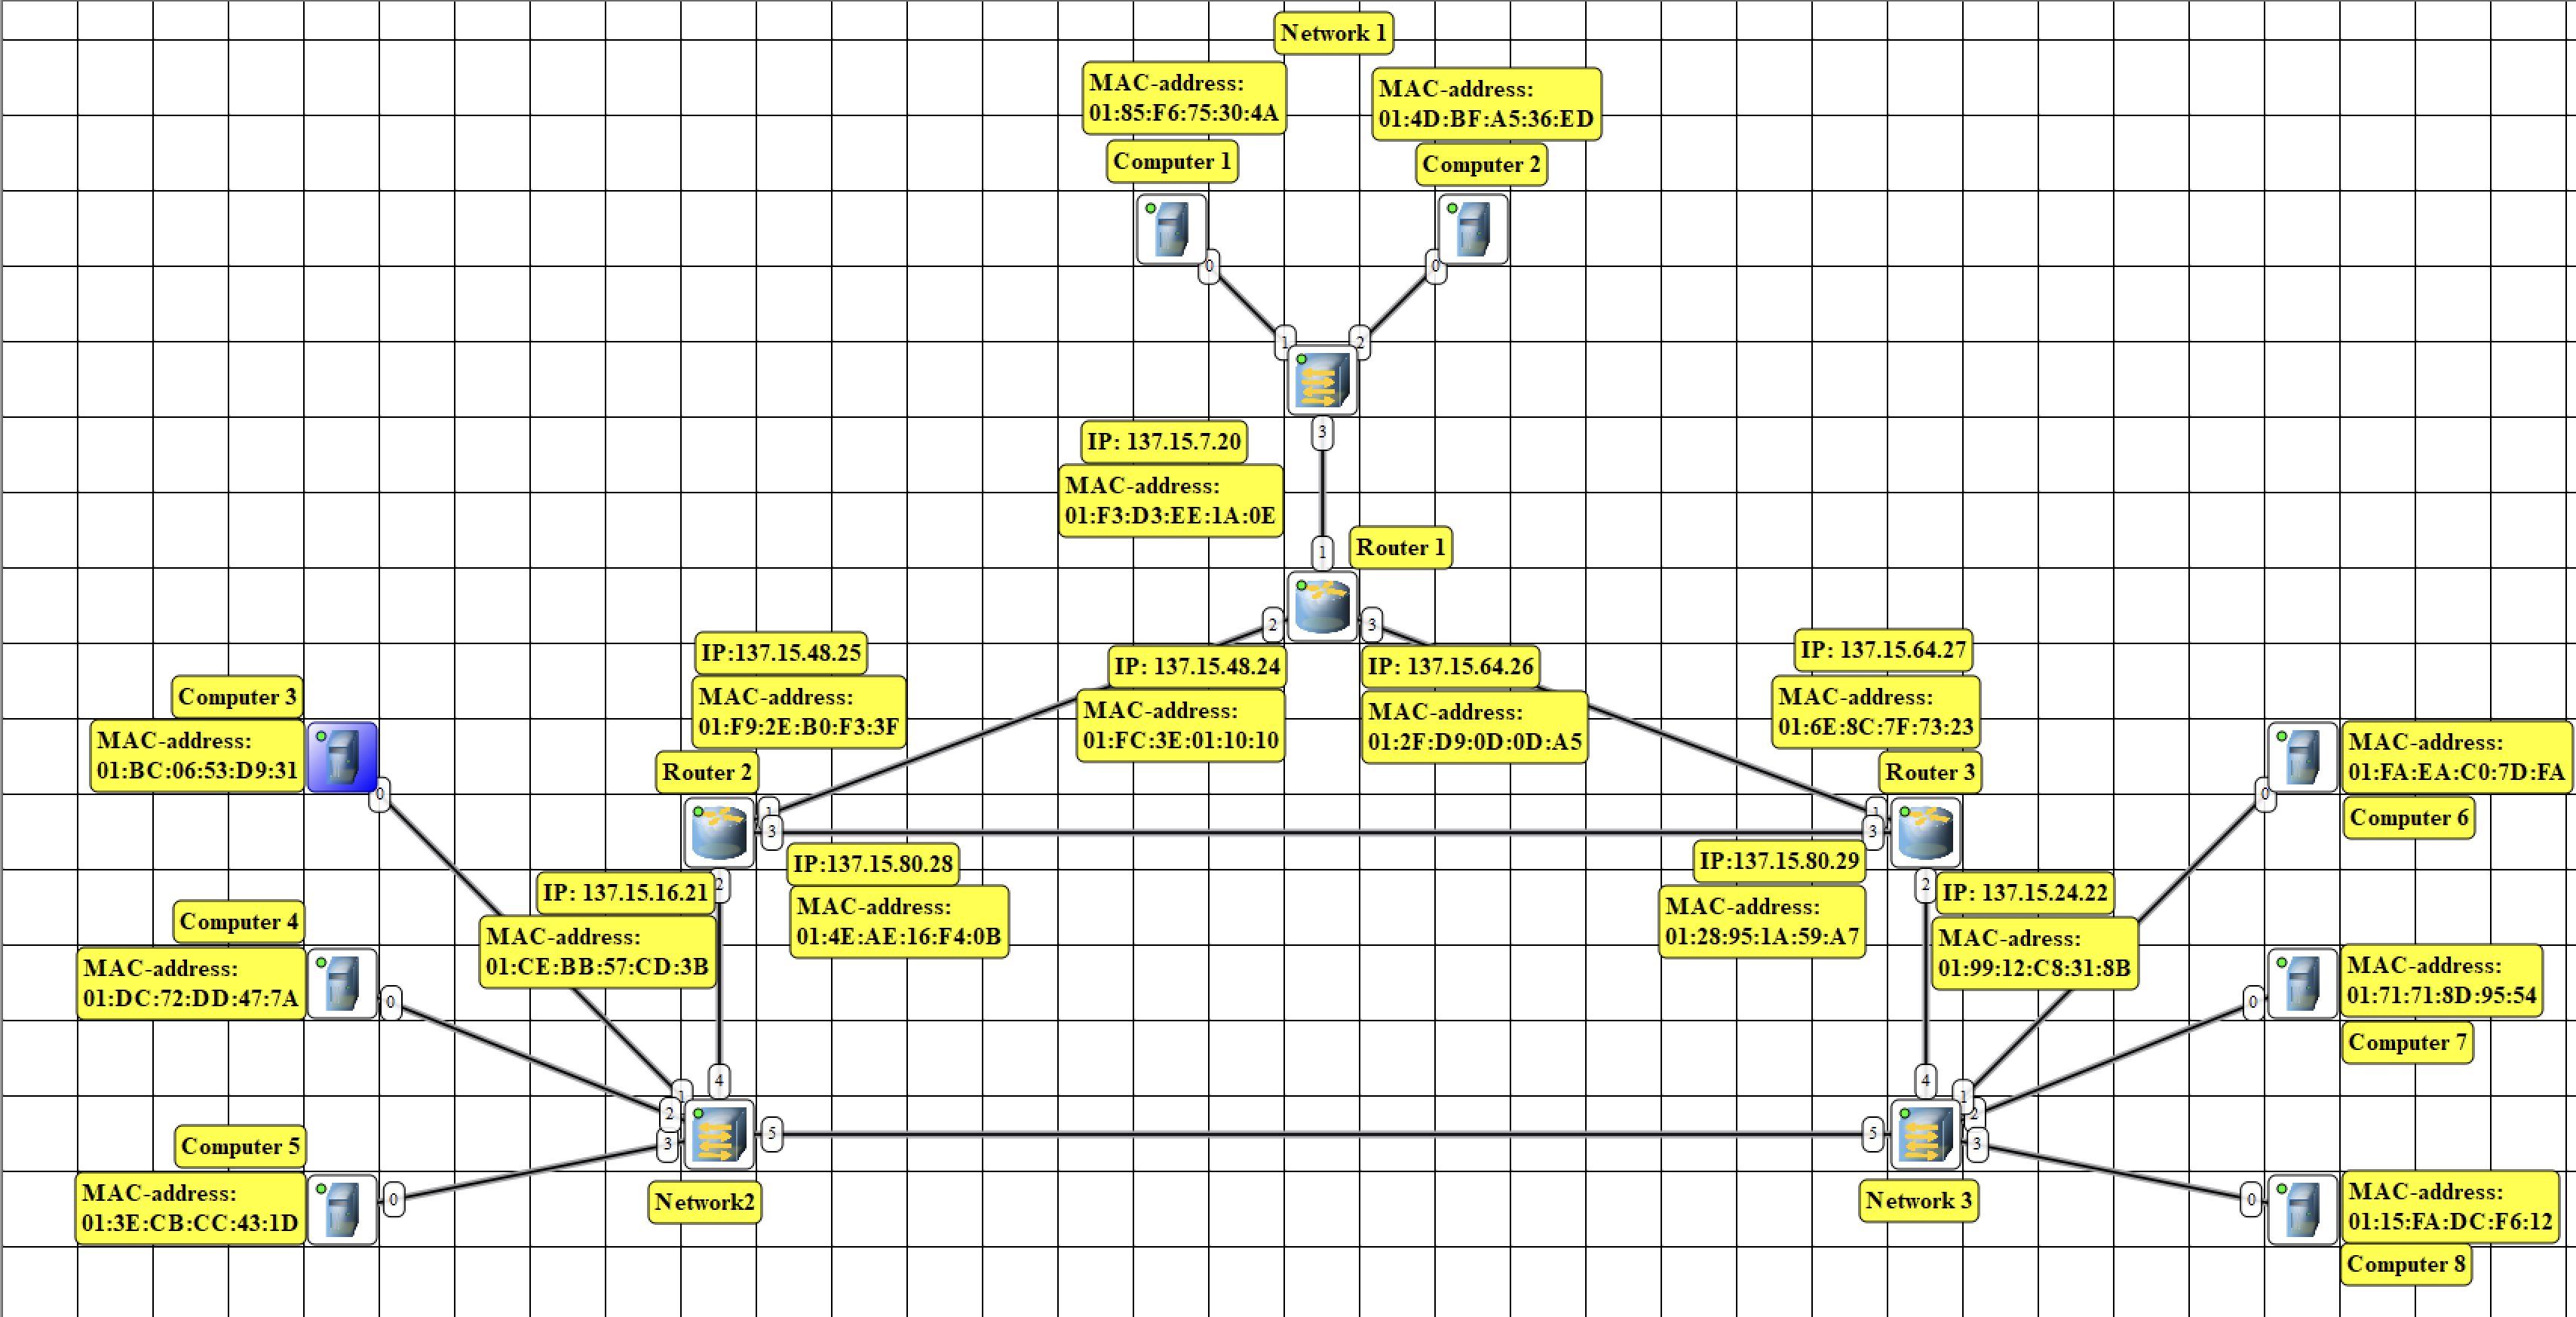
\includegraphics[width=\textwidth]{image/part-4/net5.png}
    \caption{Построенная сеть с тремя маршрутизаторами (DHCP): В5}
\end{figure}
По протоколу DHCP, компьютеры получают IP-адреса по двум разным алгоритмам: статический (соответствие MAC-адреса и IP-адреса) или из выбранного пула. В данном случае, использовался пул адресов.

Адрес выдается на ограниченный период времени (300 секунд), при этом сервер DHCP должен находиться в одной подсети с клиентом.

\begin{figure}[H]
    \centering
    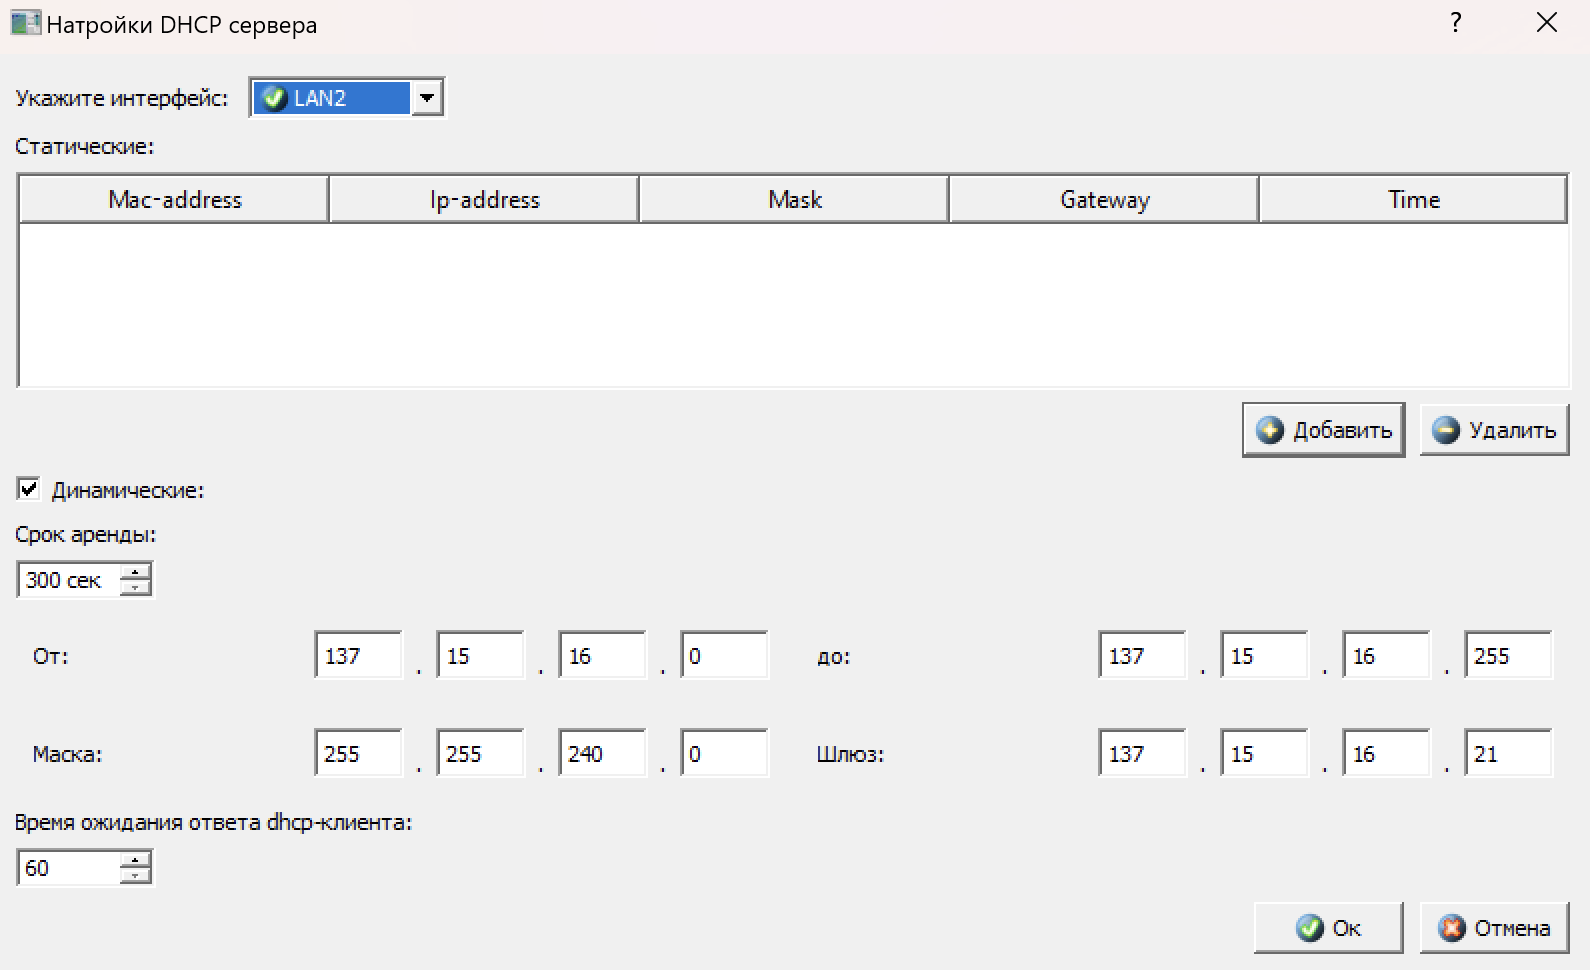
\includegraphics[width=\textwidth]{image/part-4/router2-dhcp-settings.png}
    \caption{Настройки DHCP на маршрутизаторе 2}
\end{figure}

\begin{figure}[H]
    \centering
    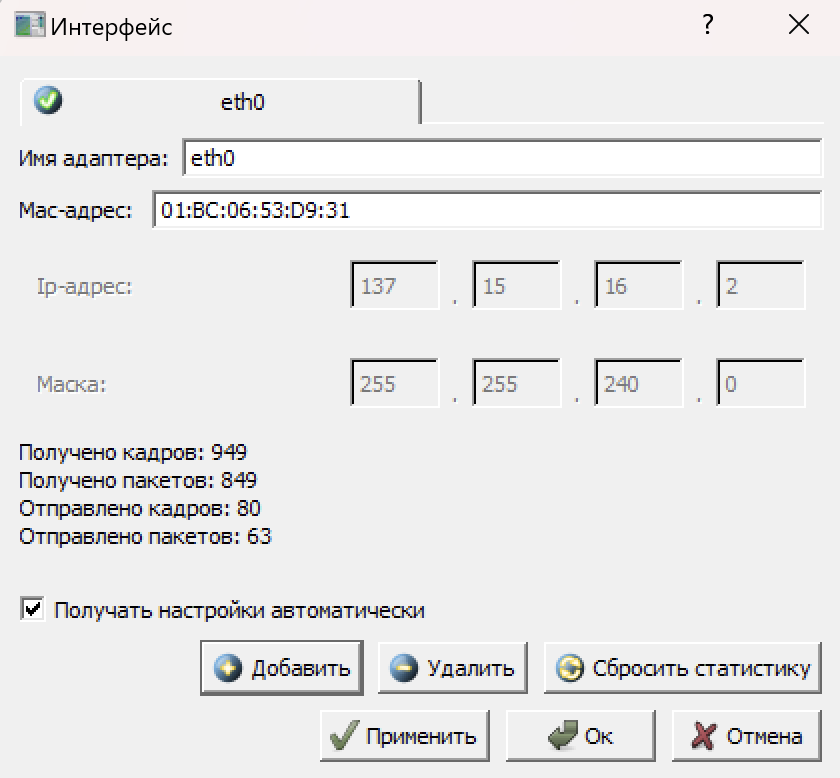
\includegraphics[width=\textwidth]{image/part-4/couputer3-ip.png}
    \caption{Получение IP-адреса на компьютере 3}
\end{figure}
\begin{figure}[H]
    \centering
    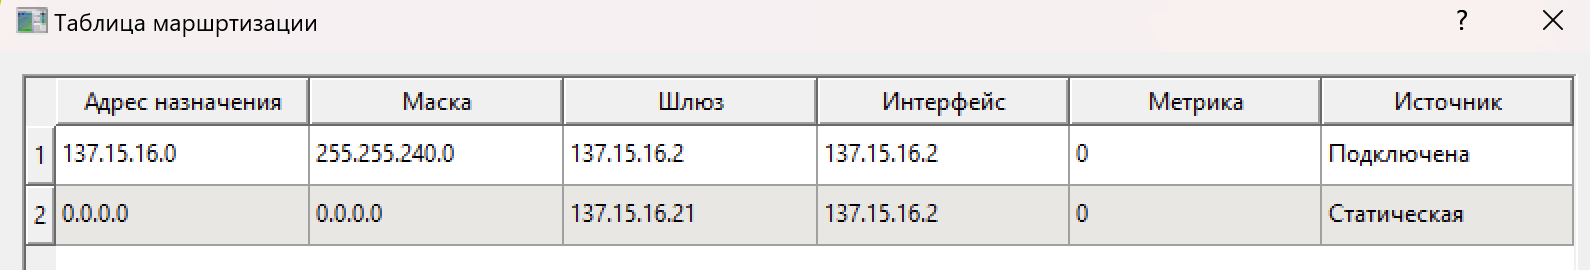
\includegraphics[width=\textwidth]{image/part-4/computer3-routing.png}
    \caption{Таблица маршрутизации компьютера 3}
\end{figure}
Принятие IP-адреса происходит в четыре этапа: DISCOVER, OFFER, REQUESI, ACK.

\begin{figure}[H]
    \centering
    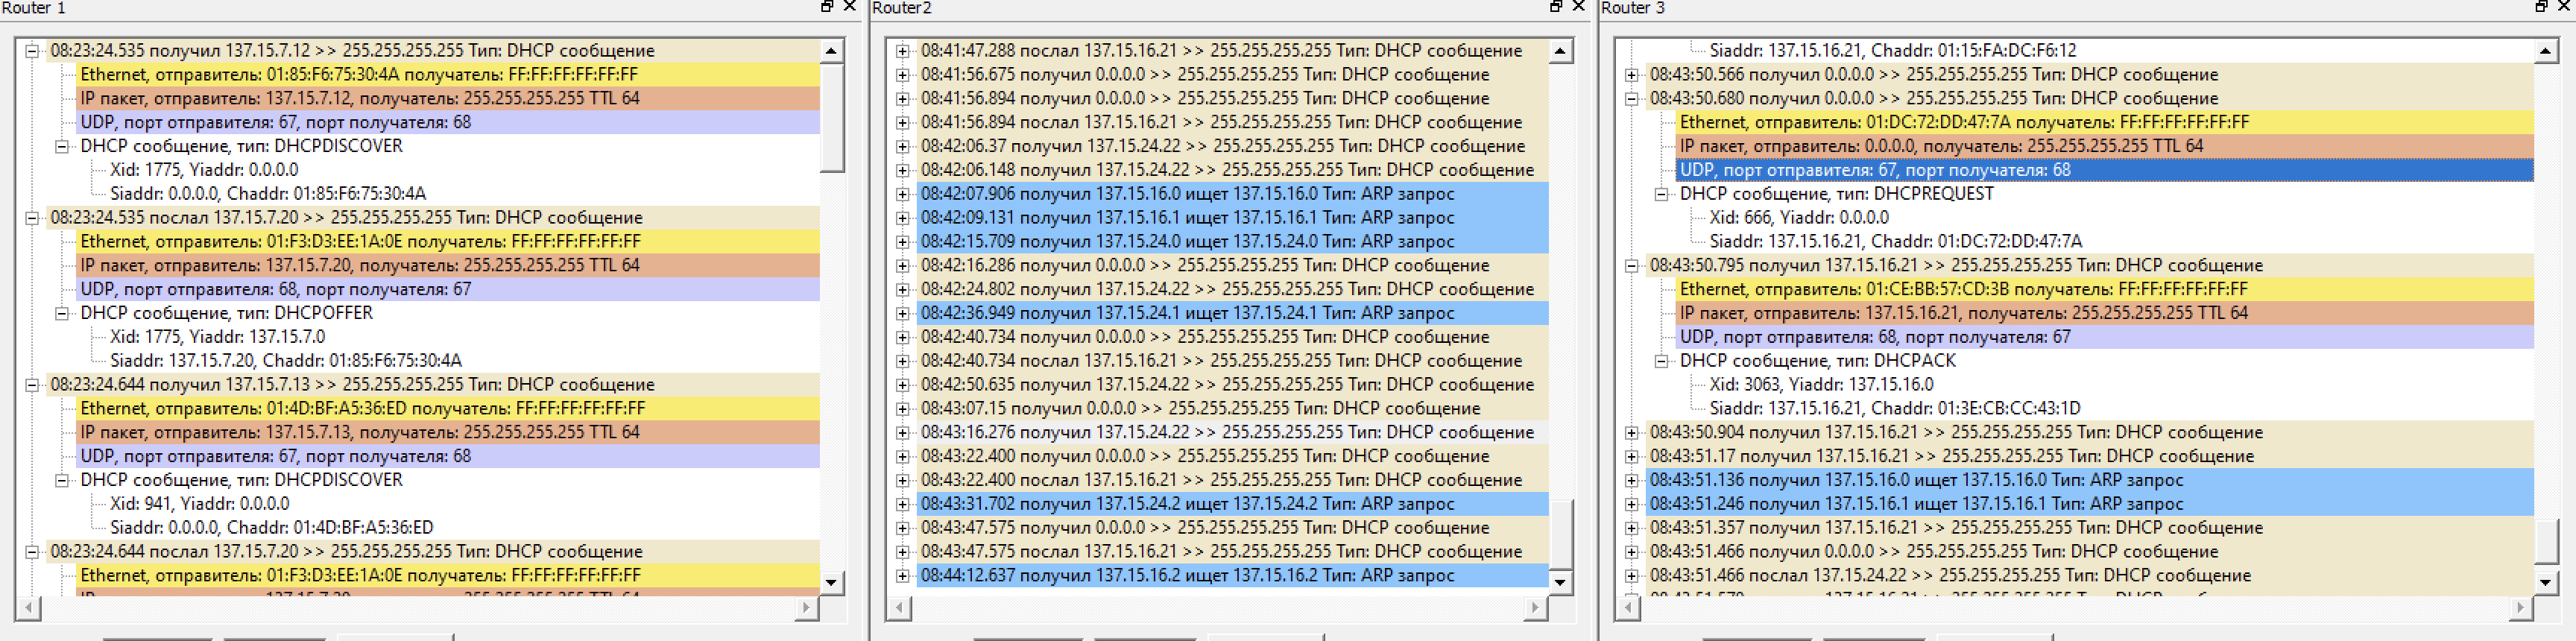
\includegraphics[width=\textwidth]{image/part-4/dhcp.png}
    \caption{Процесс работы DHCP}
\end{figure}

Механизм работы DHCP:
\begin{enumerate}
    \item Discover (поиск сервера). Когда клиент загружается в сеть, он отправляет широковещательный пакет на порт 67, который содержит сообщение DHCPDISCOVER.
     В этом сообщении содержится MAC-адрес клиента. По скольку клиент не знает подсеть к которой он относиться, то ip получателя будет 255.255.255.255. Так как у клиента ещё нет IP-адреса, то отправителем будет 0.0.0.0 и порт 68.{
            
            \includegraphics*[width=0.5\textwidth]{image/part-4/discover.png}
     }
     \item Offer (предложение сервера). Когда DHCP сервер получает сообщение DHCPDISCOVER, он резервирует доступный IP-адрес для аренды, создает запись в таблице ARP, отправляет сообщение DHCPOFFER на широковещательный адрес, которое содержит Yiaddr: предложенный адрес, Siaddr: адрес сервера, который предложил адрес, Chadddr: MAC-адрес клиента.{
        
     \includegraphics*[width=0.5\textwidth]{image/part-4/offer.png}
     }
     \item Request (запрос). Когда клиент получает сообщение DHCPOFFER, он отправляет сообщение DHCPREQUEST. Это сообщение используется как для подтверждения получения IP, так и для продления аренды. Также это сообщение служит оповещением для других DHCP серверов о отклонении их предложений. {

        \includegraphics*[width=0.5\textwidth]{image/part-4/request.png}
     }
     \item Acknowledgement (подтверждение). Когда DHCP сервер получает сообщение DHCPREQUEST, он отправляет сообщение DHCPACK, которое содержит подтверждение получения IP-адреса.{

        \includegraphics*[width=0.5\textwidth]{image/part-4/ack.png}
     }
\end{enumerate}

\section{Выводы}
В ходе выполнения лабораторной работы мы рассмотрели различные варианты построения сетей, соединения подсетей и маршрутизаторов. Также изучили принципы работы маршрутизаторов и их настройку (редактирование таблицы маршрутизации).

В первой части работы мы задавали таблицы маршрутизации маршрутизаторов статически, а затем с помощью протокола RIP, который на основе таблиц маршрутизации соседей добавлял записи в маршрутизатор с учетом количества хопов. 

Для выставления IP адресов сначала использовали статический принцип
(задавание вручную), а затем с использованием протокола DHCP и
установленных программах клиента и сервера. Данный вариант скорее
предпочтителен, если сеть часто меняется и в ней много компьютеров, однако
могут возникать проблемы с периодическим изменением IP адресов компьютеров.

\end{document}